\documentclass[letter,12pt]{article}
\usepackage[utf8]{inputenc}
\usepackage{fullpage}
\usepackage{graphicx}
\usepackage{caption}
\usepackage{subcaption}
\usepackage{datetime}
\usepackage{indentfirst}
\usepackage{wasysym}
\usepackage{placeins}

\newdateformat{mydate}{\THEDAY\space \shortmonthname[\THEMONTH] \THEYEAR}

\usepackage[backend=biber,maxbibnames=99,defernumbers=true]{biblatex}
	\addbibresource[datatype=bibtex]{Bibliography.bib}

\begin{document}

%\maketitle

\begin{flushleft}
	\begin{tabular}{l l}
		To: & Prof. Todd Kaiser \\
		From: & Sam Harkness \\
		Regarding: & EELE407 Final Report \\
		Date: & \mydate\today
	\end{tabular}
\end{flushleft}

\begin{abstract}
	This lab report details the theory and process behind fabricating CMOS logic on a silicon wafer.  
\end{abstract}

\section{Background}
	\subsection{Fabrication Theory}
		\subsubsection{Diffusion}\label{sec:Diffusion}
			\FloatBarrier
			Diffusion is a method by which doped regions of silicon are created.  A region is infused with dopants using heat and a source of dopant atoms.  In the case of wanting to create a P type silicon, our process uses Boron. In the case of N type silicon, Phosphorous is used. There are many options for dopants, but Boron and Phosphorous are some of the easier and cheaper to obtain.
			
			The rate of diffusion of a dopant depends exponentially on temperature and follow an Arrhenius behavior, as shown in Equation~\ref{eq:Diff_Coef}. $D_o$ and the activation energy $E_A$ are constants of the dopant material. $k$ is Boltzmann's constant.
			
			\begin{equation}			
				D=D_oe^{-\frac{E_A}{kT}}
				\label{eq:Diff_Coef}	
			\end{equation}
			
			Diffusion also depends on whether the source of dopants is constant or limited. As time progresses in a constant source diffusion, the concentration of dopants on the wafer remains \textbf{constant}, while the concentration inside the silicon follows a complementary error function (erfc). The impurity concentration $N$ in a constant source diffusion is determined by Equation~\ref{eq:Constant_Source_Diff}, based on time $t$ and depth $x$. $N_o$ is the surface concentration determined by the temperature of the diffusion. Figure~\ref{fig:N_o} can be used to determine $N_o$.
			
			\begin{equation}				
				N(x,t) = N_o~erfc\left(\frac{x}{2 \sqrt{D_1 t_1}}\right)
				\label{eq:Constant_Source_Diff}
			\end{equation}
			
			\begin{figure}[h]
				\centering
				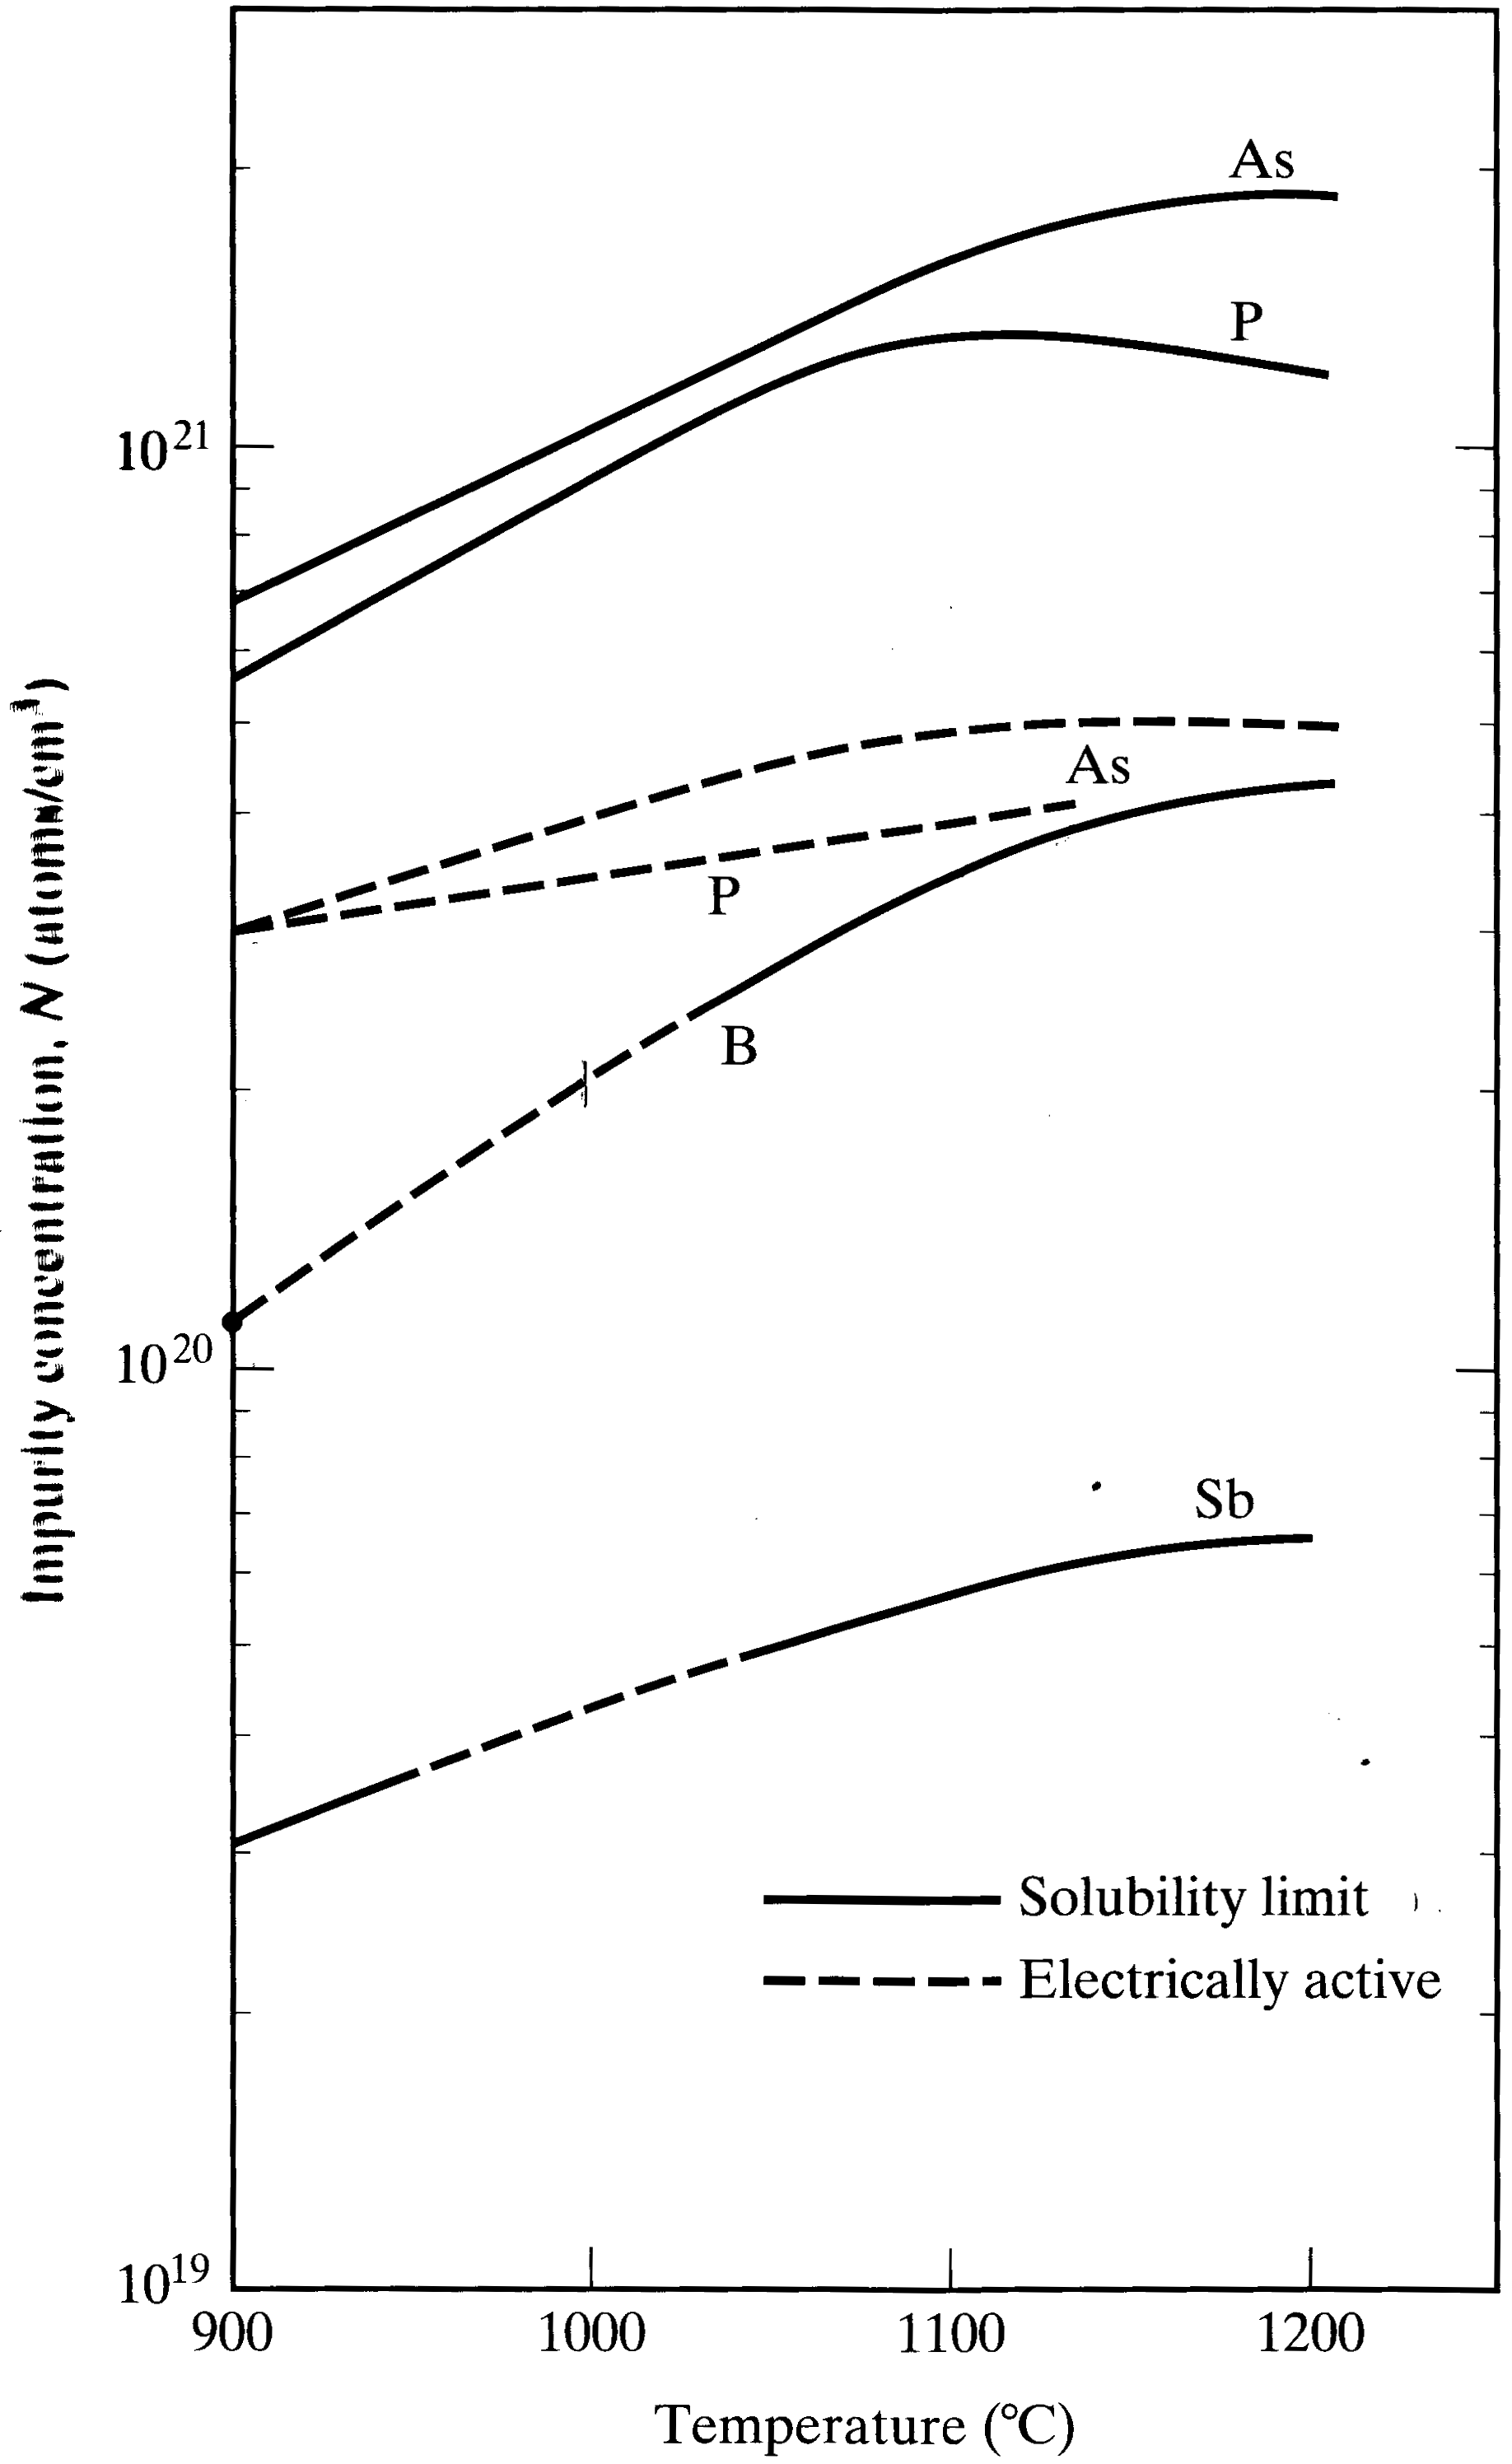
\includegraphics[scale=1]{./Images/No_Impurity_Concentration.png}
				\caption{Impurity-Concentration Limits in Si for various dopants \cite{Jaeger_02}}
				\label{fig:N_o}
			\end{figure}			
			
			A constant source diffusion is used to place a sufficient amount of dopant atoms on the surface of a wafer.  The dopant source is then removed to prevent waste of dopant atoms, while a limited-source diffusion is used to \textit{drive-in} the \textbf{limited} dopant.  The dopant remaining on the surface of the wafer before a drive-in step is calculated as the dose $Q$, as shown in Equation~\ref{eq:Dose}. The impurity concentration $N$ in a limited source diffusion is determined by Equation~\ref{eq:Limited_Source_Diff}, based on time $t$ and depth $x$.
			
			\begin{equation}			
				Q=2N_{o1}\sqrt{\frac{D_1t_1}{\pi}}
				\label{eq:Dose}	
			\end{equation}
		
			\begin{equation}			
				N(x,t) = \frac{Q}{\sqrt{\pi \sum\limits_{n} D_n t_n}}~exp\left[-\left(\frac{x}{2\sqrt{\sum\limits_{n} D_n t_n}}\right)^2\right]
				\label{eq:Limited_Source_Diff}	
			\end{equation}
			
			The final depth of a diffusion, the \textit{metallurgical junction depth} $x_j$, is useful for calculating the value of diffused resistors.  $x_j$ is calculated by setting the impurity concentration $N$ equal to the background concentration $N_B$ and solving for $x$, as shown in Equation~\ref{eq:Junction_Depth}.
			
			\begin{equation}				
				x_j=2 \sqrt{\sum\limits_{n} D_n t_n \cdot ln \frac{N_o}{N_B}}
				\label{eq:Junction_Depth}
			\end{equation}
			
			Without physically damaging the wafer, it is difficult to measure the junction depth.  However, the junction depth is directly proportional to the sheet resistance $R_s$ of the diffused region, so it can be used as a measure of accuracy of the diffusion calculations. The resistivity $\rho$ is a known constant of the substrate material. 
			
			\begin{equation}
				R_s = \frac{\rho}{x_j}
				\label{eq:Sheet_Resistance}
			\end{equation}
			
			The sheet resistance-junction depth product $R_s \cdot x_j$ can be calculated using Irvin curves. \cite{Jaeger_02}  The sheet resistance can be measured using a four-point probe, as depicted in Figure~\ref{fig:Four_Point_Probe}.
			
			\begin{figure}[h!]
				\centering
				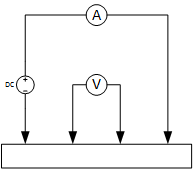
\includegraphics[scale=1]{./Images/Four_Point_Probe.png}
				\caption{Schematic of a Four-Point Probe}
				\label{fig:Four_Point_Probe}
			\end{figure}
		
		\subsubsection{Oxidation}\label{sec:Oxidation}
			\FloatBarrier
			Oxidation is the process by which an insulator is grown on a substrate; in our case Silicon Dioxide SiO$_2$ on Silicon Si. Oxidation can be performed using either a \textit{wet} or \textit{dry} process, utilizing Oxygen O$_2$ or Water H$_2$O respectively. Wet oxidation produces a worse insulator, but grows much faster.  Dry oxidation produces a better insulator, but grows much slower. Regardless of process, oxidation is modeled the same way, as shown in Equation~\ref{eq:Oxide_Thickness}.  The linear coefficient $\frac{B}{A}$ (Equation~\ref{eq:Linear_Oxidation_Coef}) and the parabolic coefficient $B$ (Equation~\ref{eq:Parabolic_Oxidation_Coef}) are both determined by an Arrhenius relationship, very similar to the diffusion coefficient as discussed in Section~\ref{sec:Diffusion}. $D_o$ and the activation energy $E_A$ are constant for the oxidation process and the type of silicon.
			
			\begin{equation}			
				X_o = \frac{A}{2}\left[-1 + \sqrt{1 + \frac{4B}{A^2}(t + \tau)}\right]
				\label{eq:Oxide_Thickness}	
			\end{equation}
		
			\begin{equation}				
				\frac{B}{A} = D_o e^{-\frac{E_A}{kT}}
				\label{eq:Linear_Oxidation_Coef}
			\end{equation}
			
			\begin{equation}				
				B = D_o e^{-\frac{E_A}{kT}}
				\label{eq:Parabolic_Oxidation_Coef}
			\end{equation}
			
			The only difference in dry vs. wet oxidation is the time offset $\tau$.  A dry oxidation behaves as if an initial oxide thickness $X_i$ of 25 nm already exists on the wafer, while a dry oxide behaves as expected with no initial oxide on the wafer.  $\tau$ can be calculated using Equation~\ref{eq:Oxide_Offset}.
			
			\begin{equation}				
				\tau = \frac{X_i^2}{B} + \frac{X_i}{B/A}
				\label{eq:Oxide_Offset}
			\end{equation}
			
			Oxide thickness can be measured using a nanospec, which utilized the reflection and refraction properties of light.
			
		\subsubsection{Photolithography}
			\FloatBarrier
			Photolithography is the process by which a mask is transmitted onto the surface of a wafer.  Photolithography is used in every step of wafer fabrication, such as oxidation, diffusion, and metal deposition. A rough estimate of the minimum feature size $F$ that can be transferred to the wafer surface is given by Equation~\ref{eq:Feature_Size}, based upon the wavelength $\lambda$ of light and the numerical aperture $NA$ of the lens. The numerical aperture of a lens is simply the sine of the convergence angle $\theta$.
		
			\begin{equation}
				F = 0.5 \frac{\lambda}{NA}
				\label{eq:Feature_Size}
			\end{equation}
			
			Also important to the photolithography process is the depth of field over which focus is maintained, given by Equation~\ref{eq:Depth_of_Field}.
			
			\begin{equation}
				DF = 0.6 \frac{\lambda}{(NA)^2}
				\label{eq:Depth_of_Field}
			\end{equation}
			
			The photoresist used in our photolithography process is Shipley 1813, a positive resist.  A positive resist is washed away in developer when exposed, whereas a negative resist is washed away in developer when not exposed. A mask is designed to be used with a certain type of resist. For this process, we use 1 $\mu$m of Shipley 1813, requiring an exposure time of 4.5 sec. To distribute an even coating of 1 $\mu$m resist, the wafer is spun at 5250 RMP for 30 sec. \cite{Shipley_1800}
		
		\subsubsection{Etching and Cleaning}
			\FloatBarrier
			Our process uses wet etching remove unwanted material, such as oxide or aluminum. SiO$_2$ is etched with Buffered Oxide Etch (BOE), a combination of hydrofluoric acid (HF) and buffering chemicals to stabilize the reaction. BOE is highly selective to silicon dioxide so the photoresist is not etched.  The only other material that needs to be etched in our process is Aluminum (Al), which is etched by Phosphoric Acid Etch (PAE) at approximately 350 \AA/min. \cite{Lab_Manual}
			
			After etching SiO$_2$ or Al, the remaining photoresist is removed using a 3 solvent clean: Acetone, Isopropyl Alcohol, and Methanol. The acetone removes the photoresist, while isopropyl and methanol remove acetone residue. Finally, the wafers are rinsed with deionized water and dried with nitrogen. This removes errant dust particles from the surface of the wafer. \cite{Lab_Manual}
			
			Before a deposition is perfomed, an RCA clean is performed. The RCA clean consists of 3 chemical solutions.  The first is a mixture of sulfuric acid and hydrogen peroxide, known as a Pirahna etch, that removes organic materials.  The second is a weak BOE to strip native oxide.  The final mixture, ionic clean, removes heavy metal ions with hydrochloric acid, water, and hydrogen peroxide. \cite{Lab_Manual}
		
		\FloatBarrier
		\subsubsection{Metal Evaporation}
			The method of depositing a conductor for this process is Physical Vapor Deposition (PVD). In our case, Aluminum (Al) is the conductor of choice for both vias and surface level connections. In PVD, the conductive material is evaporated using heat and condenses on the surface of the wafer.  Using simple geometry, the thickness of the Al can be determined for any point on the wafer.  In our case, a sheet of aluminum foil is evaporated, so we use Equation~\ref{eq:Vol_RecPrism} to find the volume of the rectangular prism.  When the Al is evaporated, the cloud of gas expands in a sphere as if it were a balloon.  The sphere of expanding gas does not contact the wafer at the same radius constant across the wafer, as seen in Figure~\ref{fig:PVD_Geometry}.
			
			\begin{equation}
				V = L \cdot W \cdot H
				\label{eq:Vol_RecPrism}
			\end{equation}
			
			\begin{figure}[h!]
				\centering
				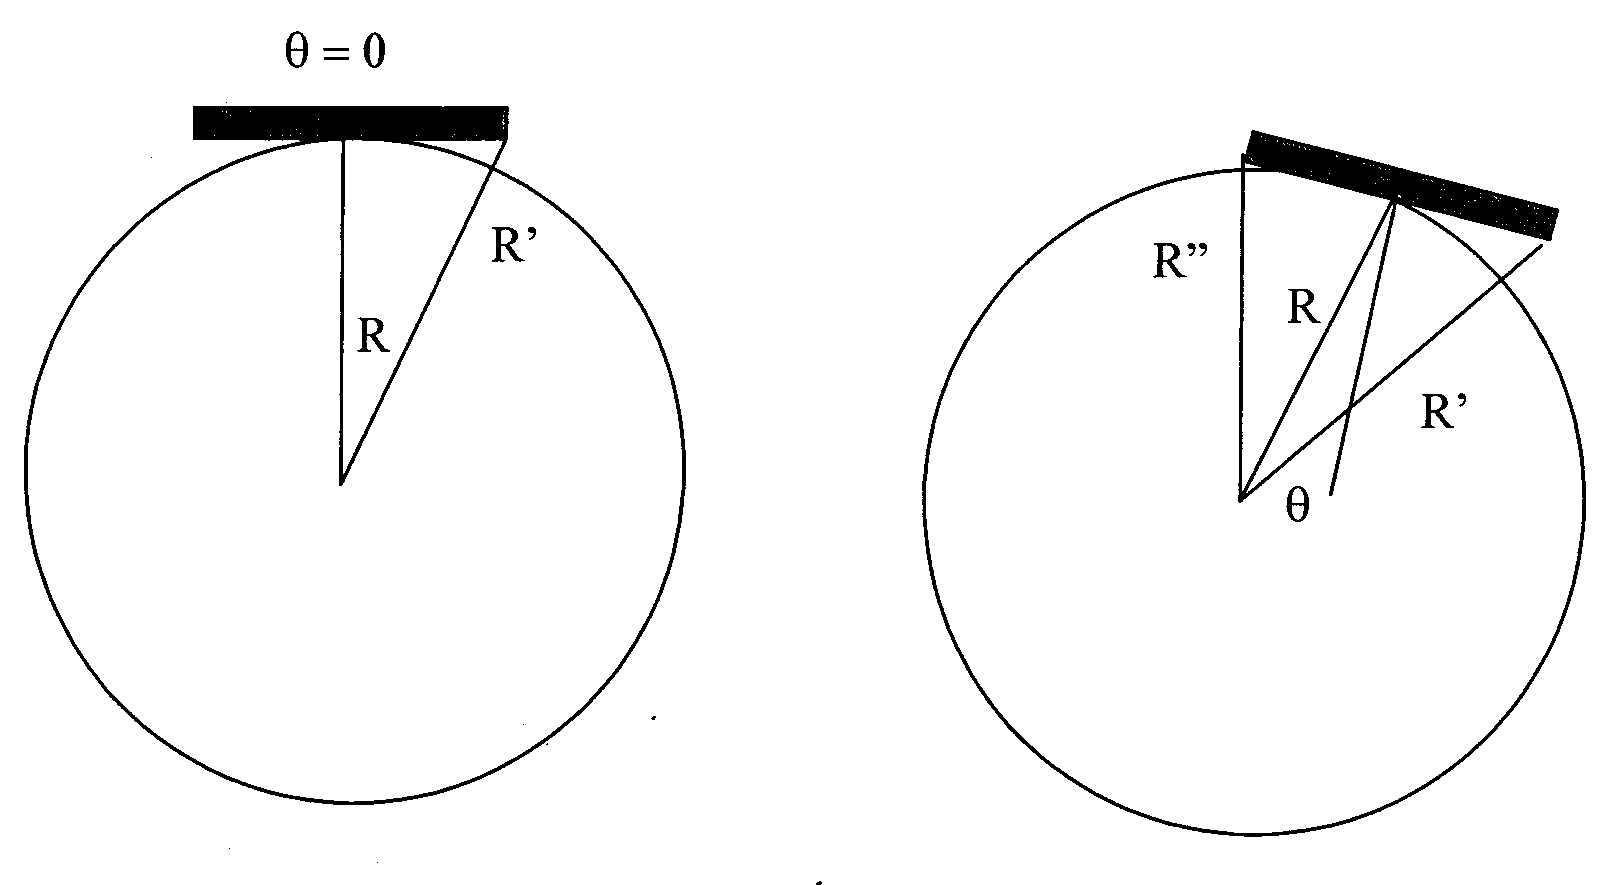
\includegraphics[width=\textwidth]{./Images/PVD_Geometry.png}
				\caption{Geometry for a PVD Step}
				\label{fig:PVD_Geometry}
			\end{figure}
			
			To determine the radius of the sphere, the law of cosines (Equation~\ref{eq:Cos_Law}) is used. After finding the various radii for the sphere, the thickness of the deposited aluminum is the volume of the evaporated material divided by the surface area of the sphere (Equation~\ref{eq:Area_Sphere}).
			
			\begin{equation}
				r^2 = b^2 + c^2 - 2bc\sin(\theta)
				\label{eq:Cos_Law}
			\end{equation}
			
			\begin{equation}
				A = 4\pi r^2
				\label{eq:Area_Sphere}
			\end{equation}				
		
	\subsection{Fabrication Sequence}
		\FloatBarrier
		The general sequence in CMOS fabrication is Oxidation, Photolithography, Deposition, Repeat. In this case, deposition refers to depositing any kind of material on the surface of the wafer, such as a dopant or conductor. Figure~\ref{fig:Fabrication_Sequence} shows the entire sequence for our process.
		
		\begin{figure}[]
			\centering
			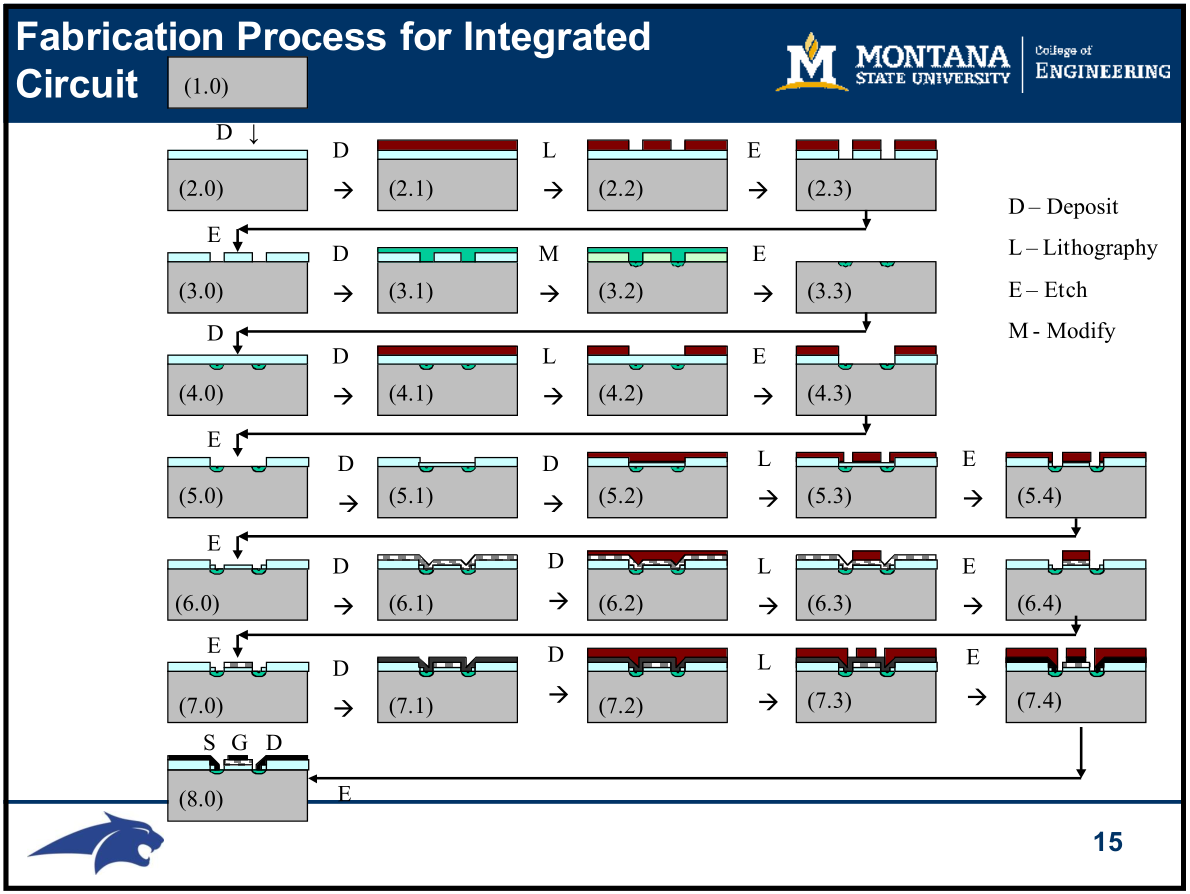
\includegraphics[width=\textwidth]{./Images/Fabrication_Sequence.png}
			\caption{Fabrication Sequence for EELE407 Process \cite{Lecture_12}}
			\label{fig:Fabrication_Sequence}
		\end{figure}

		%put a table here detailing the Fabrication Sequence
\section{Analysis}
	\subsection{Oxide Calculations}
		\FloatBarrier
		Table~\ref{tab:Oxide_Calculations} shows our calculated values for the oxide over multiple areas of the wafer, after multiple oxidations.  These values were calculated using the equations described in Section~\ref{sec:Oxidation}. 
		
		\begin{table}[]
		  \centering
		  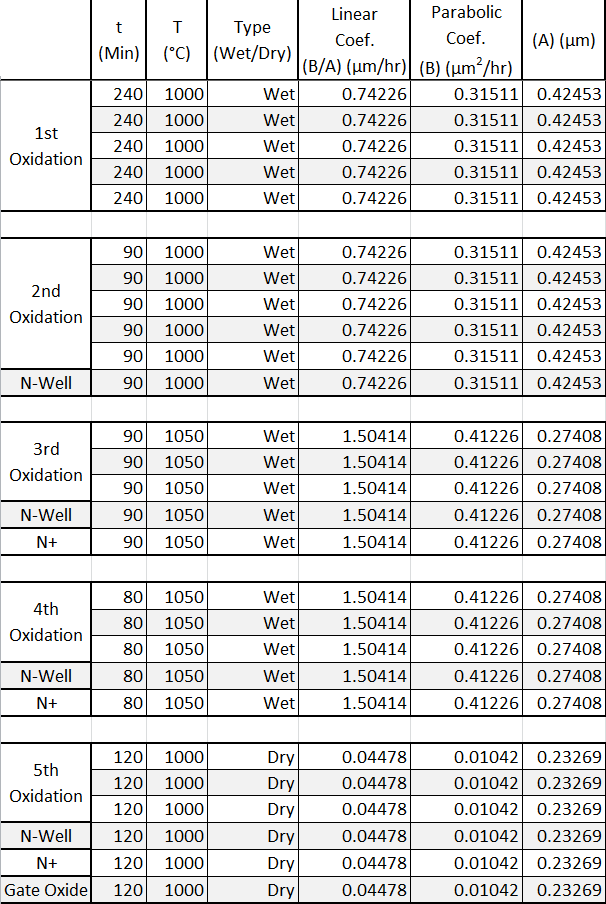
\includegraphics[scale=.75]{./Images/Oxide_Thickness_Calculations.png}
		  \caption{Oxide Calculations}
		  \label{tab:Oxide_Calculations}
		\end{table}
	
	\FloatBarrier
	\subsection{Diffusion Calculations}
		Tables~\ref{tab:N_Well_Calculations}, \ref{tab:N+_Calculations}, and \ref{tab:P+_Calculations} show the calculated and measured values for the N$^-$, N$^+$, and P$^+$ diffusions after each step of our process.  These values were calculated using the equations described in Section~\ref{sec:Diffusion}. 
		
		\begin{table}[h!]
			\centering
			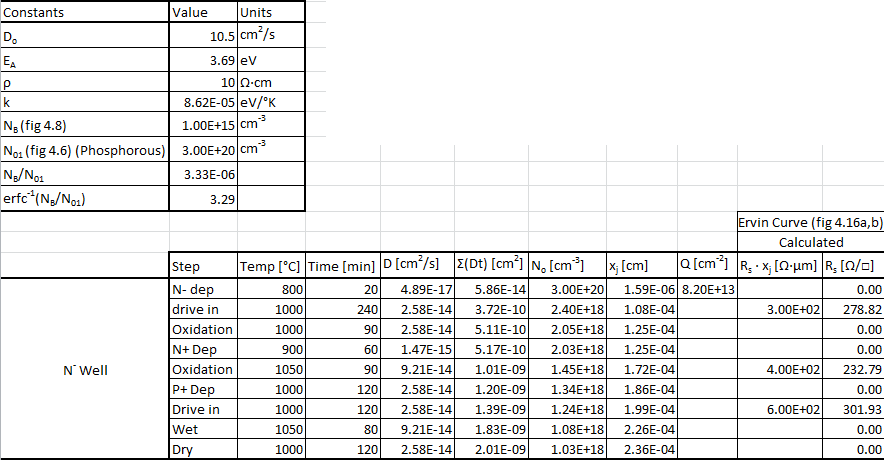
\includegraphics[width=\textwidth]{./Images/N-_Well_Calculations.png}
			\caption{N$^-$ Well Calculations}
			\label{tab:N_Well_Calculations}
		\end{table}
		
		\begin{table}[h!]
			\centering
			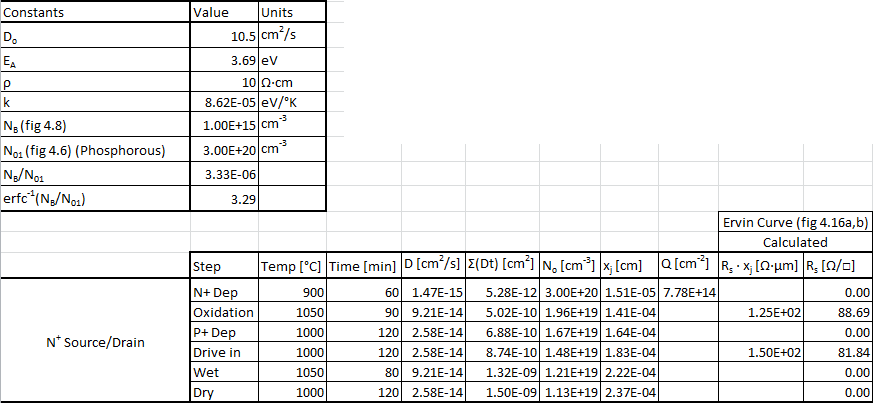
\includegraphics[width=\textwidth]{./Images/N+_Calculations.png}
			\caption{N$^+$ Source \& Drain Calculations}
			\label{tab:N+_Calculations}
		\end{table}
		
		\begin{table}[h!]
			\centering
			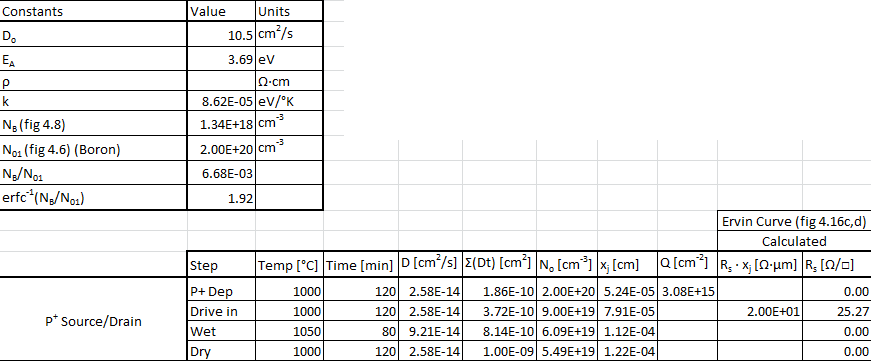
\includegraphics[width=\textwidth]{./Images/P+_Calculations.png}
			\caption{P$^+$ Source \& Drain Calculations}
			\label{tab:P+_Calculations}
		\end{table}
	
	\FloatBarrier
	\subsection{Resistor Calculations}	
		The resistivity of a material or diffusion region can be determined from its geometry and resistance. In the case of a straight line, the number of squares in the resistor is as simple as dividing the length by the width.  When 90$^\circ$ corners are added to the current path, however, an additional .56 square is added per corner. For the values in Table~\ref{tab:R_Calculations}, a corresponding graph in Figure~\ref{fig:R_Calculations} is plotted, of the form in Equation~\ref{eq:Resistance}.  The slope of the line is the resistivity of the material, while the y-axis intercept is the contact resistance.
		
		\begin{table}[]
			\centering
			\begin{subtable}[b]{.45\textwidth}
				\begin{tabular}{l | l | l | l}
					Length & Width & R & $\Box$ \\
%					[$\mu$m] & [$\mu$m] & [$\Omega$] & \hspace{12pt} \\
					\hline
					120 & 30 & 15.8 & 4.00 \\
					150 & 30 & 18.5 & 5.00 \\
					180 & 30 & 21.4 & 6.00 \\
					1300 & 30 & 109 & 43.33 \\
					2340 & 30 & 215 & 84.72 \\
					4700 & 30 & 383 & 156.67 \\
					8820 & 30 & 798 & 320.88 \\
				\end{tabular}
				\caption{Diffusion Resistors}
				\label{tab:R_Diffusion_Calculations}
			\end{subtable}
			~
			\begin{subtable}[b]{.45\textwidth}
				\begin{tabular}{l | l | l | l}
					Length & Width & R & $\Box$ \\
%					[$\mu$m] & [$\mu$m] & [$\Omega$] & \hspace{12pt} \\
					\hline
					100 & 80 & 5.2 & 1.25 \\
					100 & 40 & 5.5 & 2.50 \\
					100 & 20 & 5.8 & 5.00 \\
					1300 & 30 & 8.5 & 43.33 \\
					2340 & 30 & 12.3 & 84.72 \\
					4700 & 30 & 17.7 & 156.67 \\
					8820 & 30 & 30 & 320.88 \\
				\end{tabular}
				\caption{Metal Resistors}
				\label{tab:R_Metal_Calculations}
			\end{subtable}
			\caption{Squares Calculations given L, W, and R}
			\label{tab:R_Calculations}
		\end{table}
	
		\begin{equation}
			R = N_{sq} \cdot \rho + R_c
			\label{eq:Resistance}
		\end{equation}
	
		\begin{figure}[]
			\centering
			\begin{subfigure}[b]{.45\textwidth}
				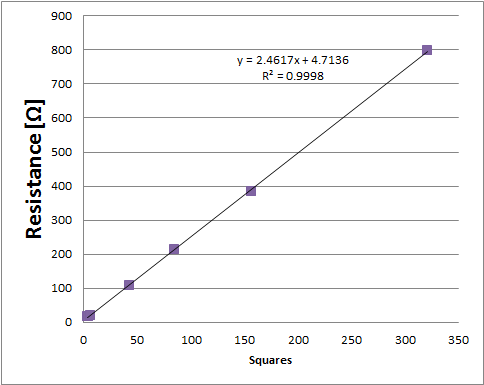
\includegraphics[width=\textwidth]{./Images/R_Diffusion_Calculations.png}
				\caption{Diffusion Resistors}
				\label{fig:R_Diffusion_Calculations}
			\end{subfigure}
			~
			\begin{subfigure}[b]{.45\textwidth}
				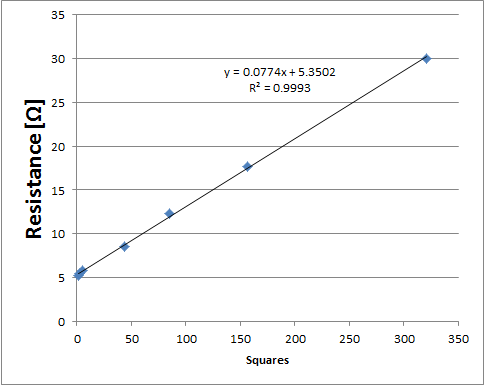
\includegraphics[width=\textwidth]{./Images/R_Metal_Calculations.png}
				\caption{Metal Resistors}
				\label{fig:R_Metal_Calculations}
			\end{subfigure}
			
			\caption{Resistivity Calculations}
			\label{fig:R_Calculations}
		\end{figure}
	
	\FloatBarrier
	\subsection{PVD Calculation}
		Our source for the PVD step was a rolled up sheet of Al foil, measuring 40 cm$^2$ by 40 $\mu$m thick, for a total volume of .16 cm$^3$. The distance from the center of the PVD chamber to the center of a mounted wafer is 13 cm. Using geometric properties and Equation~\ref{eq:Cos_Law}, we can find the distance from the center of the PVD chamber to the edges of the wafer, shown in Figure~\ref{fig:PVD_Geometry}. Our calculations find r'' to be 13.1 cm and r' to be 14.7 cm. Dividing the volume of our source by the surface area of our expanding sphere of gas, Equation~\ref{eq:Area_Sphere}, we calculate the thickness of the Al to be 753 nm at the center of the wafer, 589 nm at r', and 742 nm at r''.
		
\section{Measurements}
	\subsection{Oxide Measurements}
		\FloatBarrier
		Table~\ref{tab:Oxide_Measurements} shows the difference between the calculated and measured values of the oxide thickness, as well as the error between the calculation and measured values. Errors in the calculations can be explained by:
		\begin{itemize}
			\item Deviations from listed values (i.e. less or more time in the oxidation furnace, higher or lower temperature)
			\item Unaccounted for oxidation while the furnace is heating or cooling
			\item Natural oxide growth at room temperature
			\item Contamination of the wafer surface, inhibiting or accelerating oxidation
		\end{itemize}
		
		\begin{table}[]
			\centering
			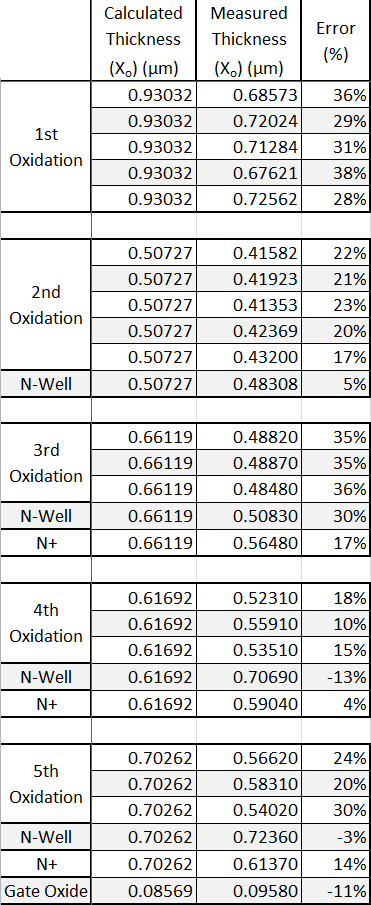
\includegraphics[scale=.75]{./Images/Oxide_Thickness_Measurements.png}
			\caption{Oxide Thickness Measurements}
			\label{tab:Oxide_Measurements}
		\end{table}
	
	\FloatBarrier
	\subsection{Sheet Resistivity}
		Tables~\ref{tab:N_Well_Measurements}, \ref{tab:N+_Measurements}, and \ref{tab:P+_Measurements} show the difference between our calculated and measured values of the sheet resistivity in the diffusion regions. Differences in measured and calculated values can be explained as:
		\begin{itemize}
			\item Deviations from listed values (i.e. less or more time in the diffusion furnace, higher or lower temperature)
			\item Unaccounted for diffusion while the furnace is heating or cooling
			\item Contamination of the wafer surface inhibiting diffusion
		\end{itemize}
		
		\begin{table}[h!]
			\centering
			\begin{tabular}{l || r | r | r || r | r}
				~ & \multicolumn{3}{c}{Calculated} & \multicolumn{2}{c}{Measured} \\
				\hline
				Step & $x_j$ [cm] & $R_s \cdot x_j [\Omega\cdot\mu m]$ & $R_s$ [$\Omega$/$\Box$] &  $R_s$ [$\Omega$/$\Box$] & $x_j$ [cm] \\
				\hline
				N$^-$ Deposition & 1.08E-04 & 3.00E+02 & 278.82 & 29.765 & 1.01E-03 \\
				N$^+$ Deposition & 1.72E-04 & 4.00E+02 & 232.79 & 34.75 & 1.15E-03 \\
				P$^+$ Deposition & 1.99E-04 & 6.00E+02 & 301.93 & 56.55 & 1.06E-03 \\
			\end{tabular}
			\caption{N$^-$ Well Measurements}
			\label{tab:N_Well_Measurements}
		\end{table}
	
		\begin{table}[h!]
			\centering
			\begin{tabular}{l || r | r | r || r | r}
				~ & \multicolumn{3}{c}{Calculated} & \multicolumn{2}{c}{Measured} \\
				\hline
				Step & $x_j$ [cm] & $R_s \cdot x_j [\Omega\cdot\mu m]$ & $R_s$ [$\Omega$/$\Box$] &  $R_s$ [$\Omega$/$\Box$] & $x_j$ [cm] \\
				\hline
				N$^+$ Deposition & 1.41E-04 & 1.25E+02 & 88.69 & 28.1 & 4.45E-04 \\
				P$^+$ Deposition & 1.83E-04 & 1.50E+02 & 81.84 & 2.675 & 5.61E-03 \\
			\end{tabular}
			\caption{N$^+$ Source \& Drain Measurements}
			\label{tab:N+_Measurements}
		\end{table}

		\begin{table}[h!]
			\centering
			\begin{tabular}{l || r | r | r || r | r}
				~ & \multicolumn{3}{c}{Calculated} & \multicolumn{2}{c}{Measured} \\
				\hline
				Step & $x_j$ [cm] & $R_s \cdot x_j [\Omega\cdot\mu m]$ & $R_s$ [$\Omega$/$\Box$] &  $R_s$ [$\Omega$/$\Box$] & $x_j$ [cm] \\
				\hline
				P$^+$ Deposition & 7.91E-05 & 2.00E+01 & 25.27 & 34.65 & 5.77E-05 \\
			\end{tabular}
			\caption{P$^+$ Source \& Drain Measurements}
			\label{tab:P+_Measurements}
		\end{table}
			
	\FloatBarrier
	\subsection{Aluminum Thickness}
		Figure~\ref{fig:Al_Thickness} shows the thickness of the aluminum on the surface of the wafer after etching. The thickness of the patterned aluminum is measured using a profilometer. The height of the aluminum and silicon are both averaged to removed local maximums and minimums, leading to a measured thickness of 417 nm of aluminum. This deviates from our worst case calculated value of 589 nm possibly because of:
		\begin{itemize}
			\item Loss of Al on the surface of the heating element
			\item Less Al was evaporated than in the calculation
		\end{itemize}
		
		\begin{figure}[h!]
			\centering
			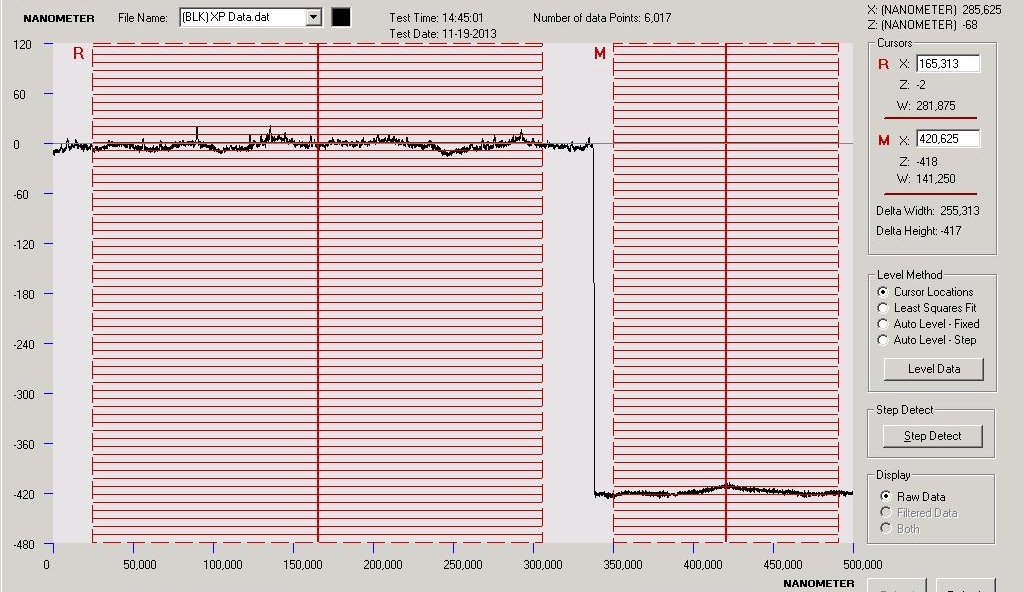
\includegraphics[width=\textwidth]{./Images/Harkness_Step.jpg}
			\caption{Aluminum Thickness}
			\label{fig:Al_Thickness}
		\end{figure}

\clearpage
\FloatBarrier
\section{Device Testing}
	\subsection{Resistors}
		Figure~\ref{fig:R_Image} shows resistors on the surface of our wafer before and after the Al Deposition step.  Figures~\ref{fig:R_Metal_Measurements}, \ref{fig:R_NPlus_Measurements}, \ref{fig:R_PPlus_Measurements}, and \ref{fig:R_Tub_Measurements} show plots of $R(V)$ and $I(V)$. $R(V)$ could also be derived as the slope of $I(V)$. 
	
		\begin{figure}[h!]
			\centering
			\begin{subfigure}[b]{.45\textwidth}
				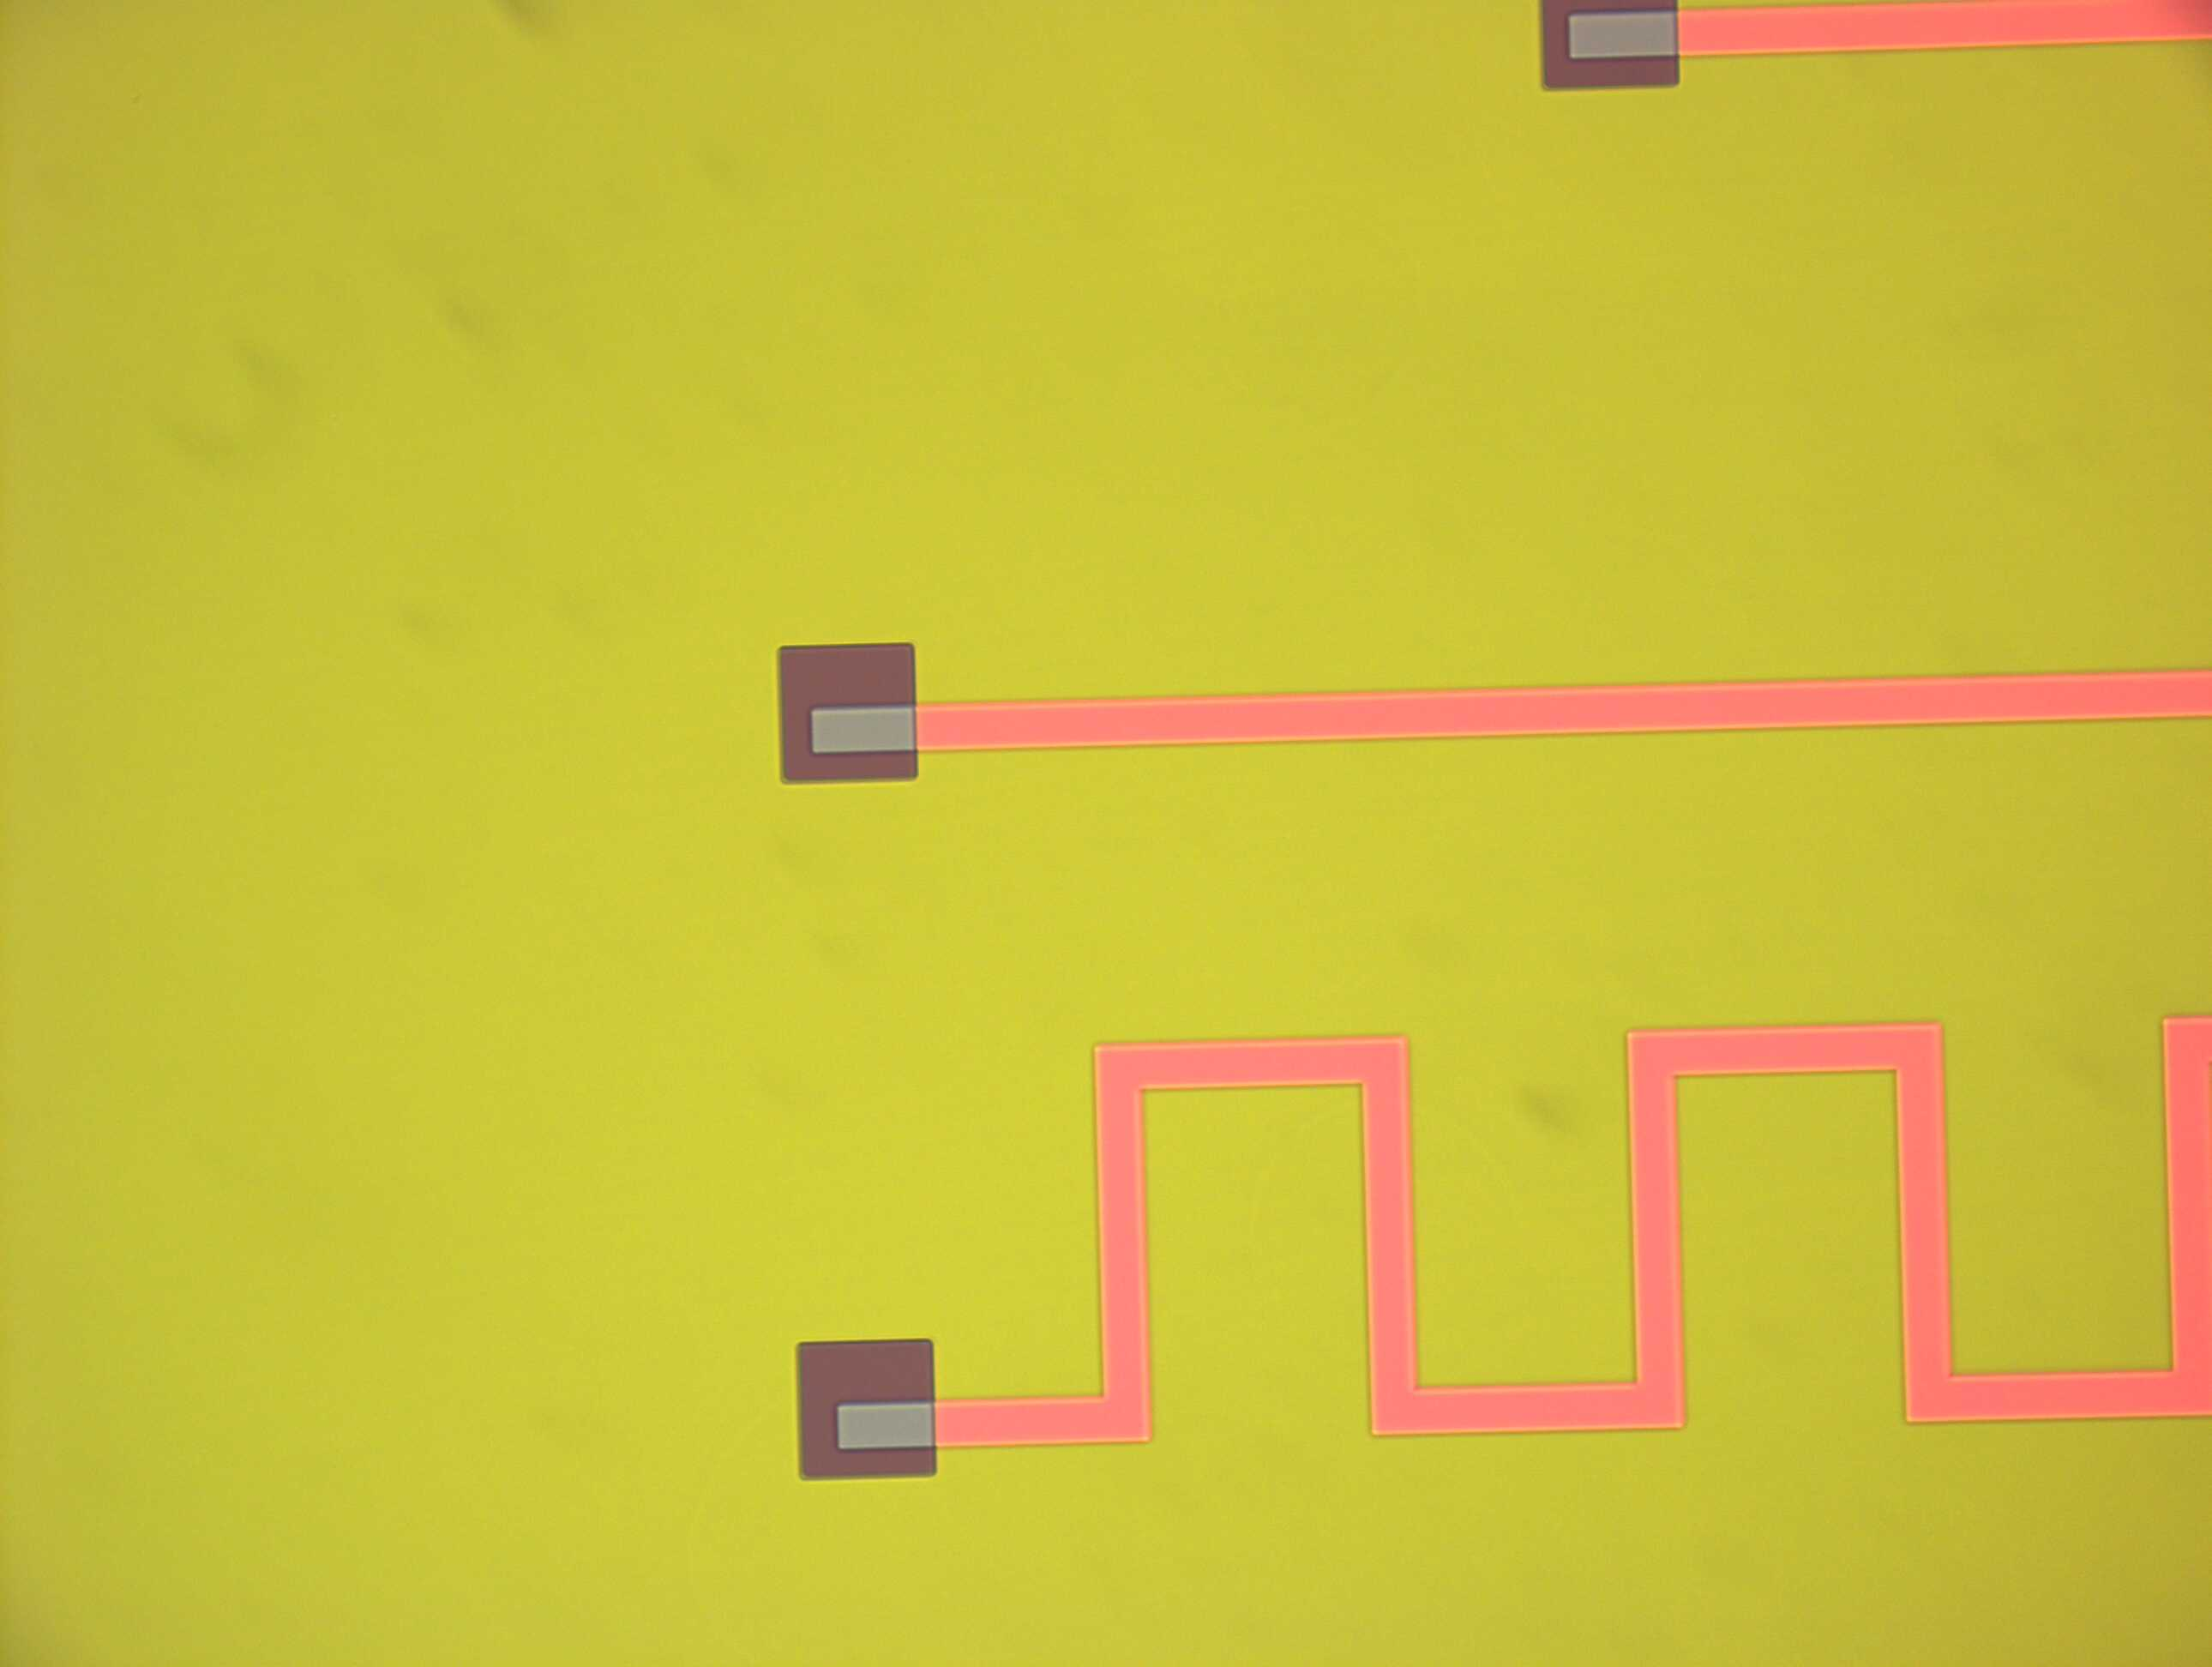
\includegraphics[width=\textwidth]{./Images/5_Nov_Resistors.jpg}
				\caption{Diffusion Resistors before Al Deposition}
			\end{subfigure}
			~
			\begin{subfigure}[b]{.45\textwidth}
				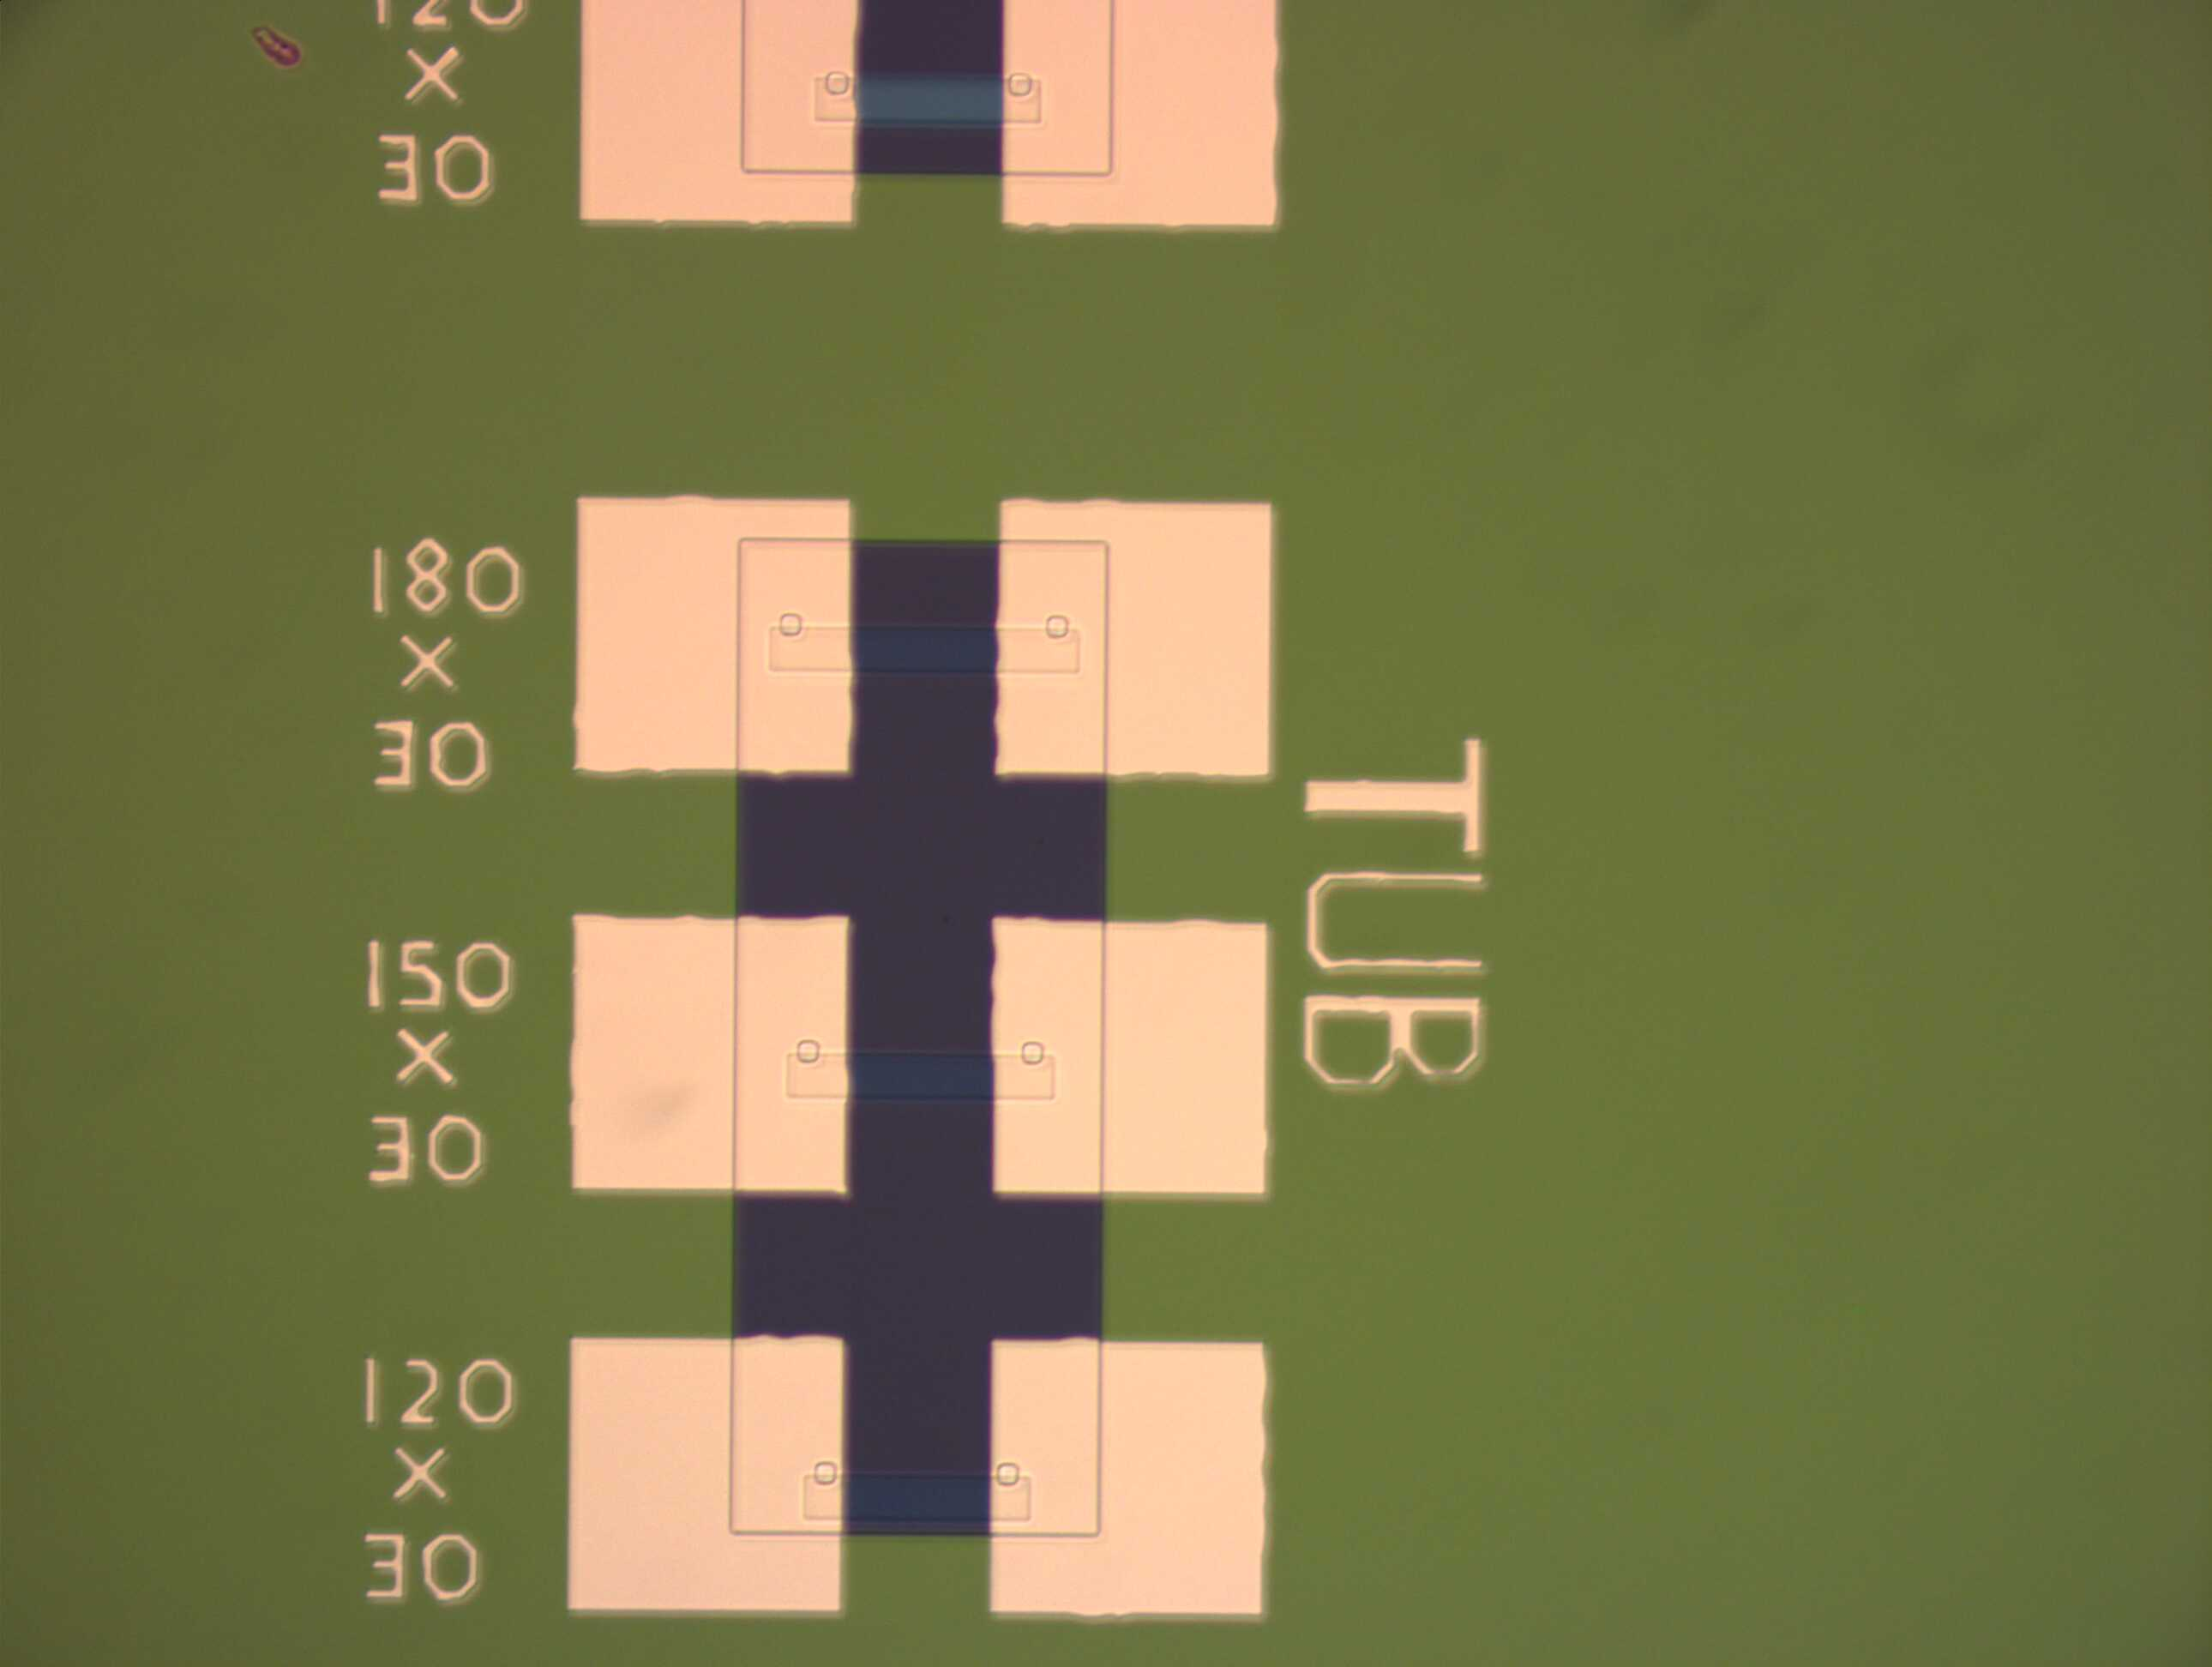
\includegraphics[width=\textwidth]{./Images/19_Nov_Resistors.jpg}
				\caption{Diffusion Resistors after Al Deposition}
			\end{subfigure}
			\caption{Captured Images of Resistors}
			\label{fig:R_Image}
		\end{figure}
		
		\pagebreak
		\FloatBarrier
		\subsubsection{Metal}
			Of special note are the metal resistors.  Due to the low impedance of the aluminum traces, the tester very quickly reaches its current limiting parameter of 100 mA. The resistance value displayed after this point is reached is not accurate. Instead, the true value of the resistor is the value when the slope of $R(V)$ is 0.
		
			\begin{figure}[h!]
				\centering
				\begin{subfigure}[b]{.45\textwidth}
					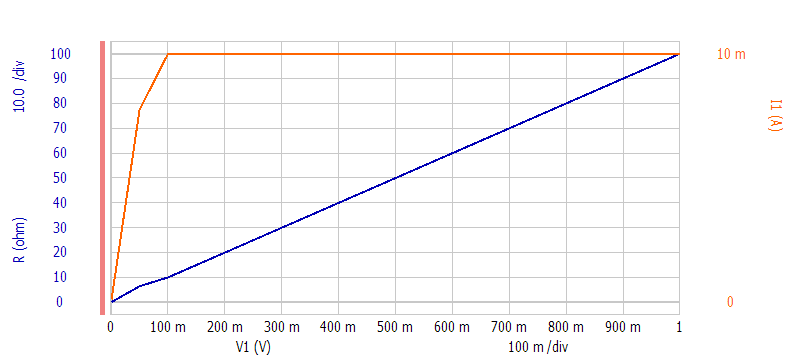
\includegraphics[width=\textwidth]{./Images/Probe_Test/R_Metal_100x20.png}
					\caption{2.5 $\Omega$ Metal 100x20}
				\end{subfigure}
				~
				\begin{subfigure}[b]{.45\textwidth}
					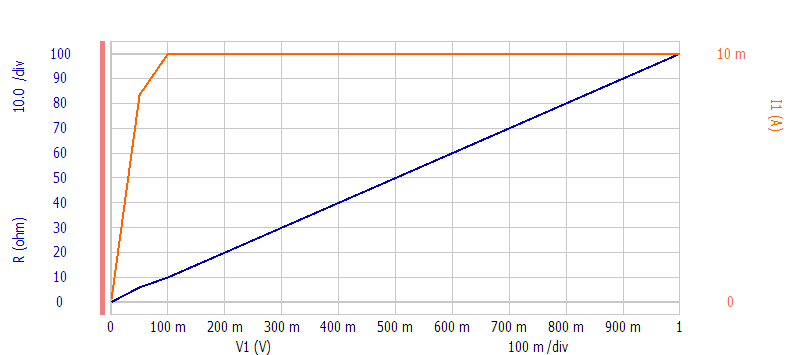
\includegraphics[width=\textwidth]{./Images/Probe_Test/R_Metal_100x40.png}
					\caption{3.33 $\Omega$ Metal 100x40}
				\end{subfigure}
				~
				\begin{subfigure}[b]{.45\textwidth}
					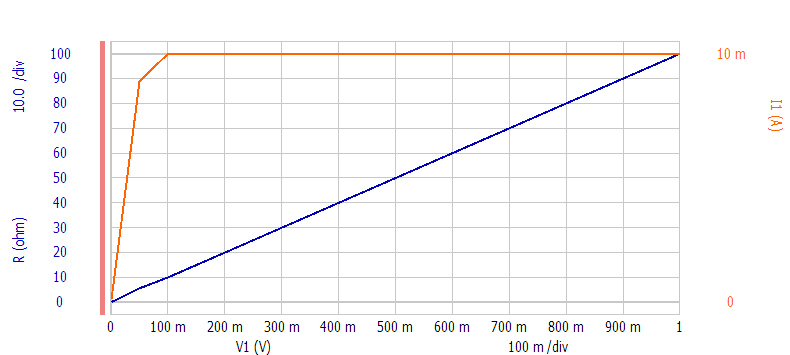
\includegraphics[width=\textwidth]{./Images/Probe_Test/R_Metal_100x80.png}
					\caption{5 $\Omega$ Metal 100x80}
				\end{subfigure}
				~
				\begin{subfigure}[b]{.45\textwidth}
					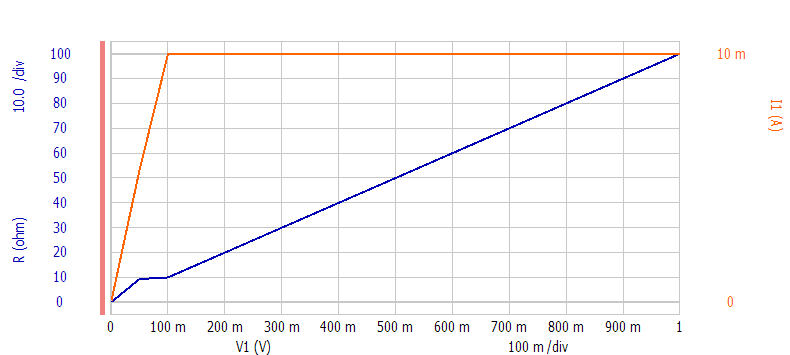
\includegraphics[width=\textwidth]{./Images/Probe_Test/R_Metal_1300x30.png}
					\caption{10 $\Omega$ Metal 1300x30}
				\end{subfigure}
				~
				\begin{subfigure}[b]{.45\textwidth}
					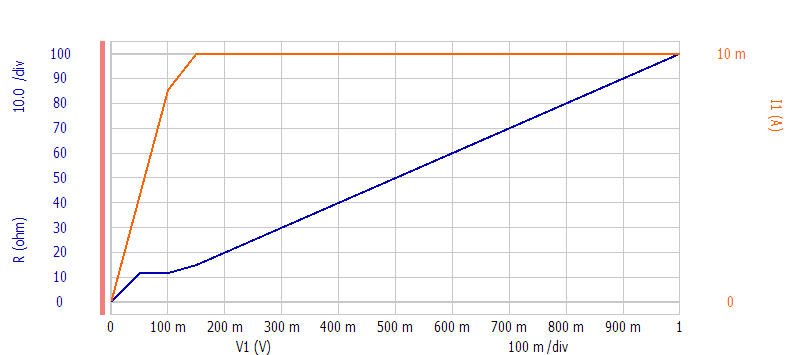
\includegraphics[width=\textwidth]{./Images/Probe_Test/R_Metal_2340x30.png}
					\caption{12.5 $\Omega$ Metal 2340x30}
				\end{subfigure}
				~
				\begin{subfigure}[b]{.45\textwidth}
					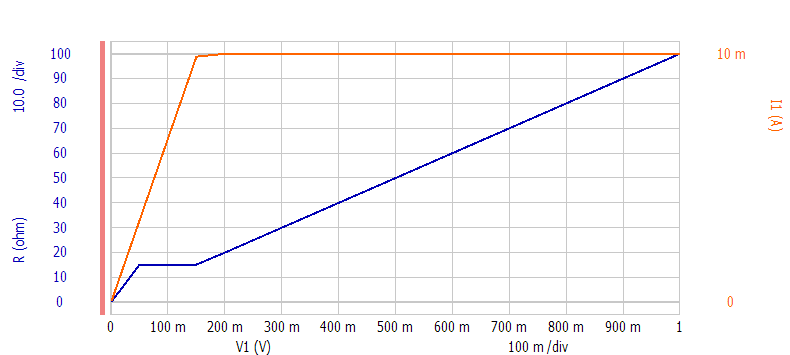
\includegraphics[width=\textwidth]{./Images/Probe_Test/R_Metal_4700x30.png}
					\caption{15 $\Omega$ Metal 4700x30}
				\end{subfigure}
				~
				\begin{subfigure}[b]{.45\textwidth}
					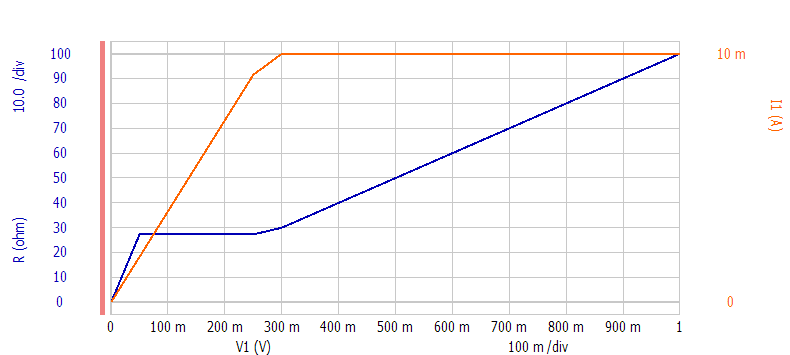
\includegraphics[width=\textwidth]{./Images/Probe_Test/R_Metal_8820x30.png}
					\caption{27.5 $\Omega$ Metal 8820x30}
				\end{subfigure}
				\caption{Metal Resistor Measurements}
				\label{fig:R_Metal_Measurements}
			\end{figure}
		
		\FloatBarrier	
		\subsubsection{N$^+$}
			The resistance of the resistors in Figure~\ref{fig:R_NPlus_Measurements} must be estimated in some cases, because the resistances never reach a steady state.  In this case, it is easiest to estimate the slope of the current plot.
			
			\begin{figure}[h!]
				\centering
				\begin{subfigure}[b]{.45\textwidth}
					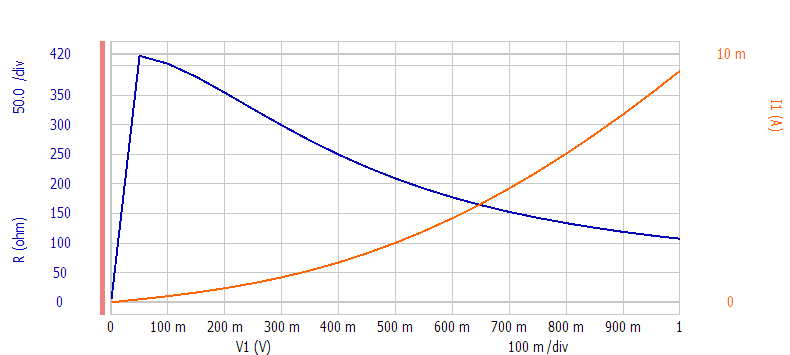
\includegraphics[width=\textwidth]{./Images/Probe_Test/R_NPlus_120x30.png}
					\caption{75 $\Omega$ N$^+$ 120x30}
				\end{subfigure}
				~
				\begin{subfigure}[b]{.45\textwidth}
					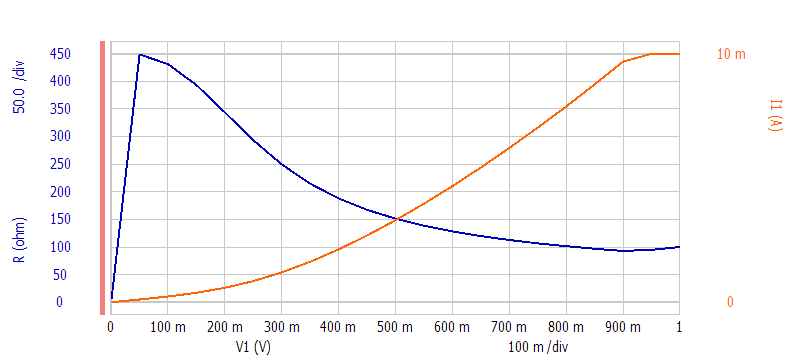
\includegraphics[width=\textwidth]{./Images/Probe_Test/R_NPlus_150x30.png}
					\caption{95 $\Omega$ N$^+$ 150x30}
				\end{subfigure}
				~
				\begin{subfigure}[b]{.45\textwidth}
					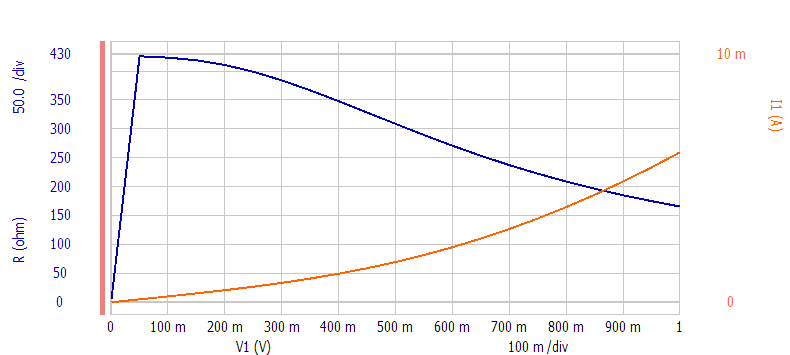
\includegraphics[width=\textwidth]{./Images/Probe_Test/R_NPlus_180x30.png}
					\caption{100 $\Omega$ N$^+$ 180x30}
				\end{subfigure}
				~
				\begin{subfigure}[b]{.45\textwidth}
					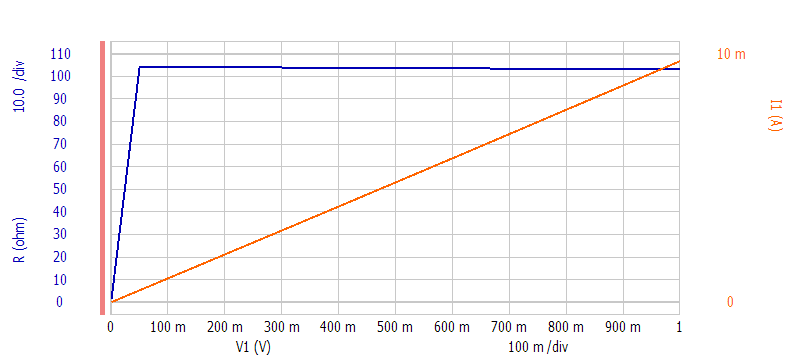
\includegraphics[width=\textwidth]{./Images/Probe_Test/R_NPlus_1300x30.png}
					\caption{103 $\Omega$ N$^+$ 1300x30}
				\end{subfigure}
				~
				\begin{subfigure}[b]{.45\textwidth}
					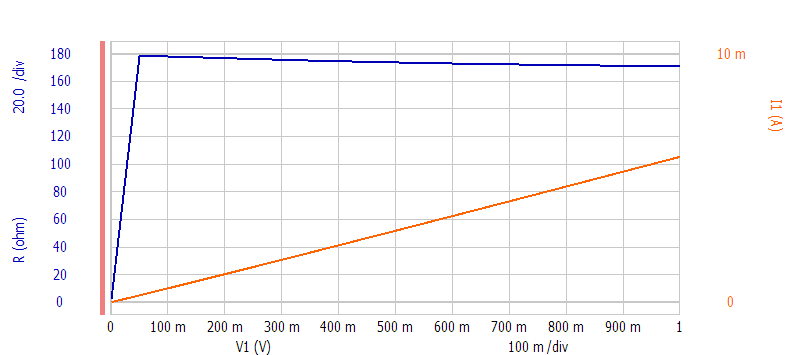
\includegraphics[width=\textwidth]{./Images/Probe_Test/R_NPlus_2340x30.png}
					\caption{170 $\Omega$ N$^+$ 2340x30}
				\end{subfigure}
				~
				\begin{subfigure}[b]{.45\textwidth}
					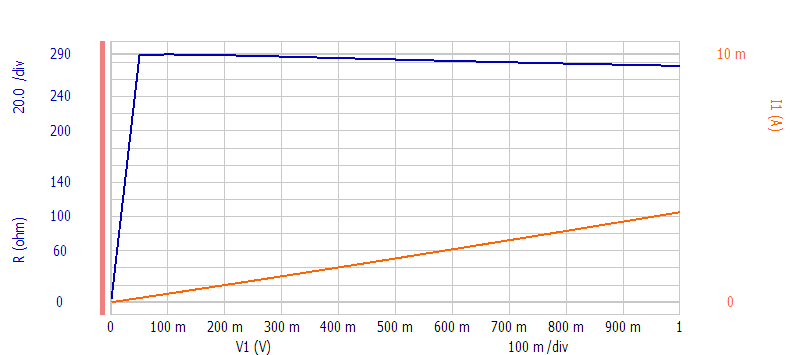
\includegraphics[width=\textwidth]{./Images/Probe_Test/R_NPlus_4700x30.png}
					\caption{280 $\Omega$ N$^+$ 4700x30}
				\end{subfigure}
				~
				\begin{subfigure}[b]{.45\textwidth}
					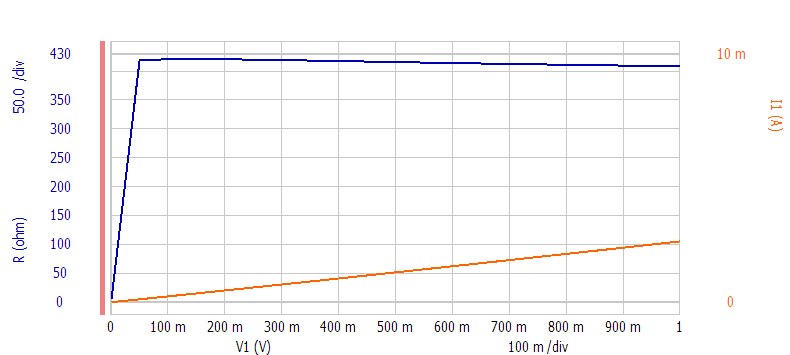
\includegraphics[width=\textwidth]{./Images/Probe_Test/R_NPlus_8820x30.png}
					\caption{410 $\Omega$ N$^+$ 8820x30}
				\end{subfigure}
				\caption{N$^+$ Resistor Measurements}
				\label{fig:R_NPlus_Measurements}
			\end{figure}
		
		\FloatBarrier	
		\subsubsection{P$^+$}
			The 2340x30 resistor in Figure~\ref{fig:R_PPlus_Measurements} should have greater resistance than the 1300x30 resistor because of its increased length.  The same holds true for the 8820x30 resistor compared to the 4700x30 resistor.  These discrepancies may be the result of contamination on the wafer, or an increased contact resistance between the resistors.
			
			\begin{figure}[h!]
				\centering
				\begin{subfigure}[b]{.45\textwidth}
					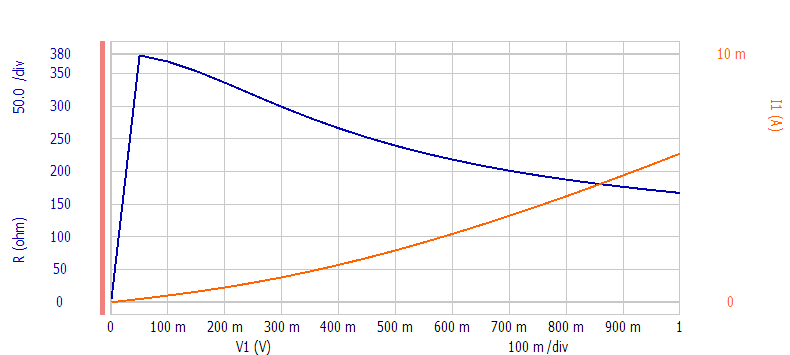
\includegraphics[width=\textwidth]{./Images/Probe_Test/R_PPlus_120x30.png}
					\caption{160$\Omega$ P$^+$ 120x30}
				\end{subfigure}
				~
				\begin{subfigure}[b]{.45\textwidth}
					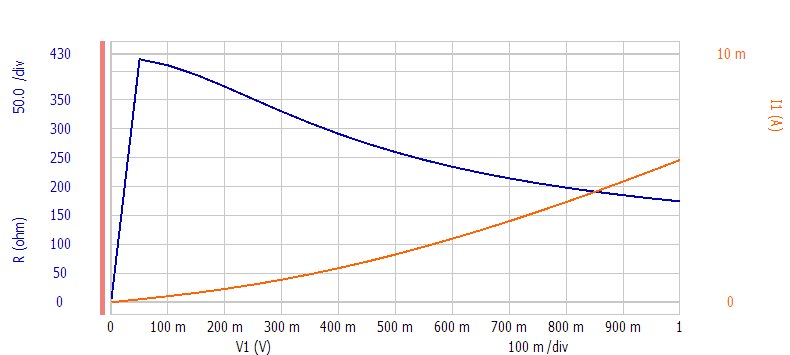
\includegraphics[width=\textwidth]{./Images/Probe_Test/R_PPlus_150x30.png}
					\caption{170$\Omega$ P$^+$ 150x30}
				\end{subfigure}
				~
				\begin{subfigure}[b]{.45\textwidth}
					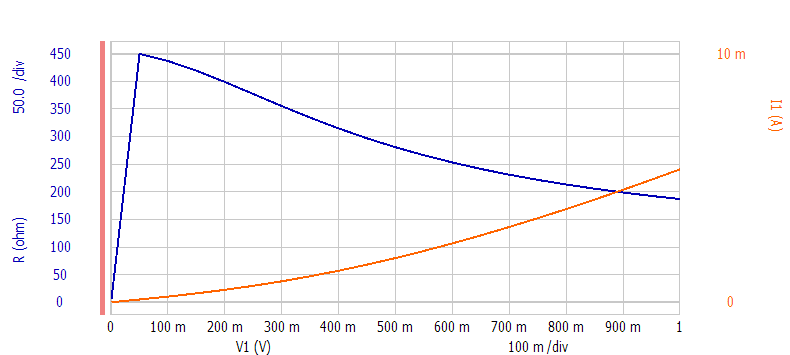
\includegraphics[width=\textwidth]{./Images/Probe_Test/R_PPlus_180x30.png}
					\caption{180 $\Omega$ P$^+$ 180x30}
				\end{subfigure}
				~
				\begin{subfigure}[b]{.45\textwidth}
					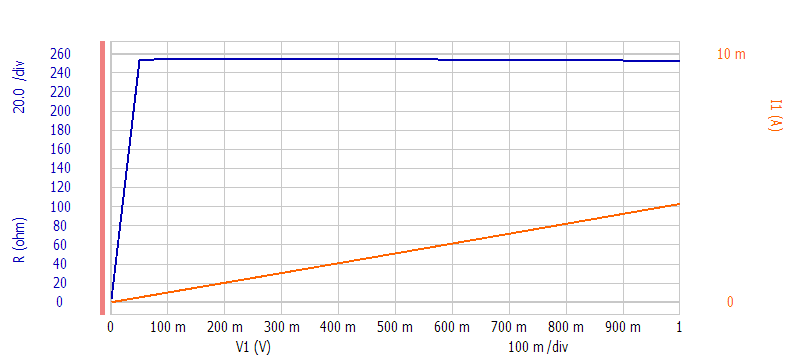
\includegraphics[width=\textwidth]{./Images/Probe_Test/R_PPlus_1300x30.png}
					\caption{250 $\Omega$ P$^+$ 1300x30}
				\end{subfigure}
				~
				\begin{subfigure}[b]{.45\textwidth}
					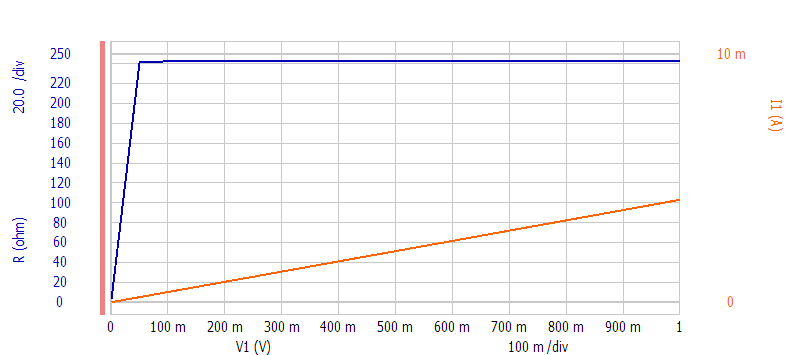
\includegraphics[width=\textwidth]{./Images/Probe_Test/R_PPlus_2340x30.png}
					\caption{240 $\Omega$ P$^+$ 2340x30}
				\end{subfigure}
				~
				\begin{subfigure}[b]{.45\textwidth}
					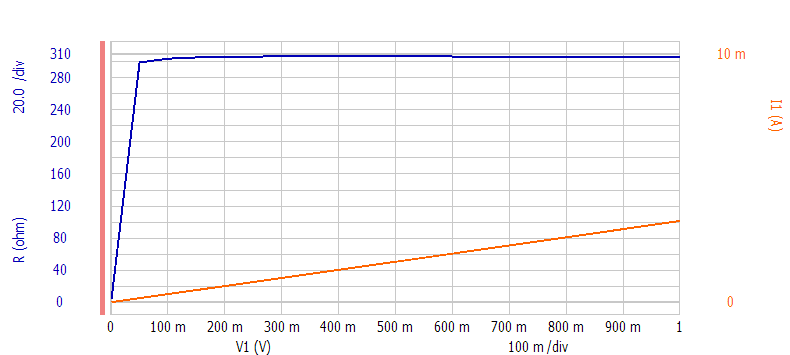
\includegraphics[width=\textwidth]{./Images/Probe_Test/R_PPlus_4700x30.png}
					\caption{310 $\Omega$ P$^+$ 4700x30}
				\end{subfigure}
				~
				\begin{subfigure}[b]{.45\textwidth}
					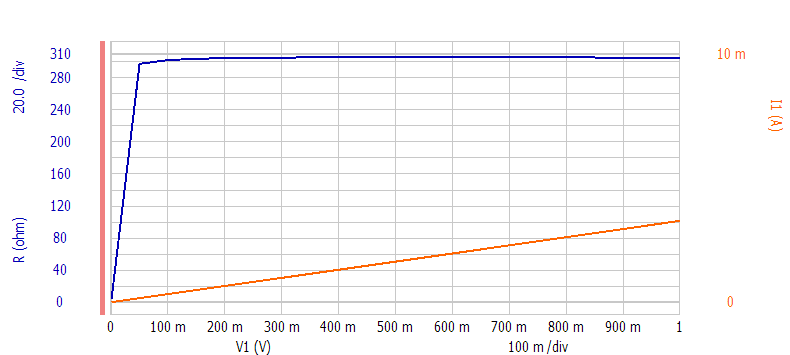
\includegraphics[width=\textwidth]{./Images/Probe_Test/R_PPlus_8820x30.png}
					\caption{310 $\Omega$ P$^+$ 8820x30}
				\end{subfigure}
				\caption{P$^+$ Resistor Measurements}
				\label{fig:R_PPlus_Measurements}
			\end{figure}
		
		\FloatBarrier	
		\subsubsection{N$^-$ Well (Tub)}
			The N$^-$ Well resistors have some of the same discrepancies as the P$^+$ resistors, likely for the same reasons, such as wafer contamination or contact resistance.
					
			\begin{figure}[h!]
				\centering
				\begin{subfigure}[b]{.45\textwidth}
					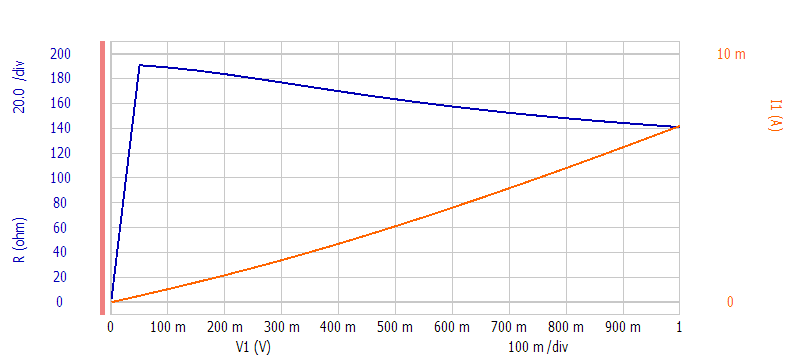
\includegraphics[width=\textwidth]{./Images/Probe_Test/R_Tub_120x30.png}
					\caption{140 $\Omega$ N$^-$ 120x30}
				\end{subfigure}
				~
				\begin{subfigure}[b]{.45\textwidth}
					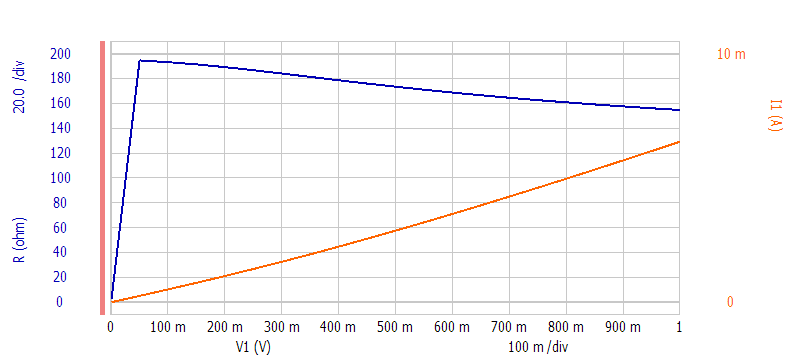
\includegraphics[width=\textwidth]{./Images/Probe_Test/R_Tub_150x30.png}
					\caption{155 $\Omega$ N$^-$ 150x30}
				\end{subfigure}
				~
				\begin{subfigure}[b]{.45\textwidth}
					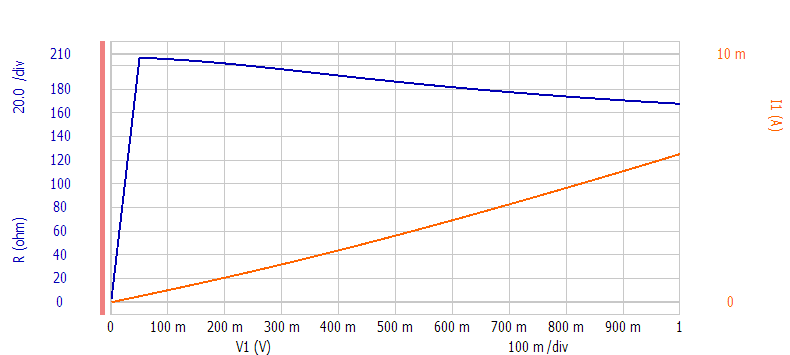
\includegraphics[width=\textwidth]{./Images/Probe_Test/R_Tub_180x30.png}
					\caption{165 $\Omega$ N$^-$ 180x30}
				\end{subfigure}
				~
				\begin{subfigure}[b]{.45\textwidth}
					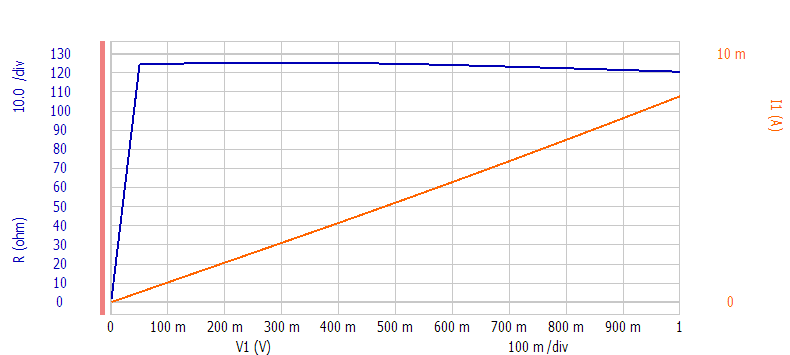
\includegraphics[width=\textwidth]{./Images/Probe_Test/R_Tub_1300x30.png}
					\caption{120 $\Omega$ N$^-$ 1300x30}
				\end{subfigure}
				~
				\begin{subfigure}[b]{.45\textwidth}
					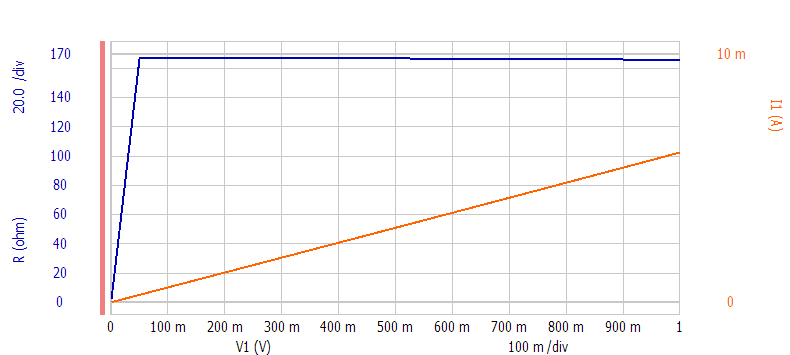
\includegraphics[width=\textwidth]{./Images/Probe_Test/R_Tub_2340x30.png}
					\caption{165 $\Omega$ N$^-$ 2340x30}
				\end{subfigure}
				~
				\begin{subfigure}[b]{.45\textwidth}
					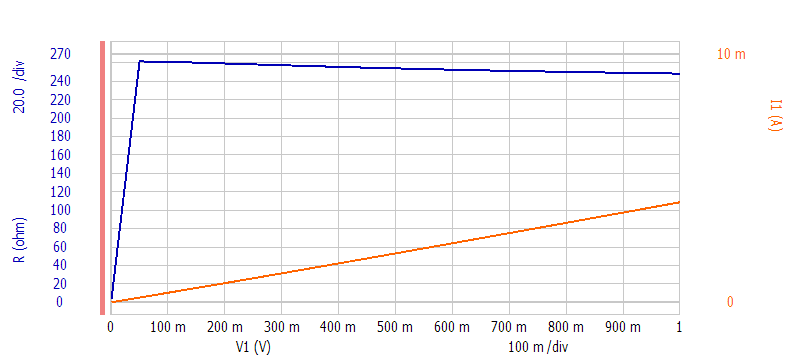
\includegraphics[width=\textwidth]{./Images/Probe_Test/R_Tub_4700x30.png}
					\caption{250 $\Omega$ N$^-$ 4700x30}
				\end{subfigure}
				~
				\begin{subfigure}[b]{.45\textwidth}
					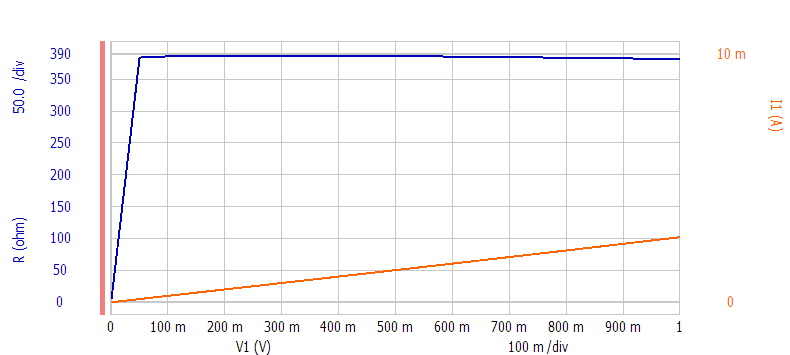
\includegraphics[width=\textwidth]{./Images/Probe_Test/R_Tub_8820x30.png}
					\caption{385 $\Omega$ N$^-$ 8820x30}
				\end{subfigure}
				\caption{N$^-$ Resistor Measurements}
				\label{fig:R_Tub_Measurements}
			\end{figure}
	
	\FloatBarrier		
	\subsection{Diodes}	
		Figure~\ref{fig:D_Image} shows some of the diodes created in our process.  Figures~\ref{fig:D_1diff} and \ref{fig:D_2diff} show plots for both the 1 diffusion and 2 diffusion diodes.
		
		\begin{figure}[h!]
			\centering
			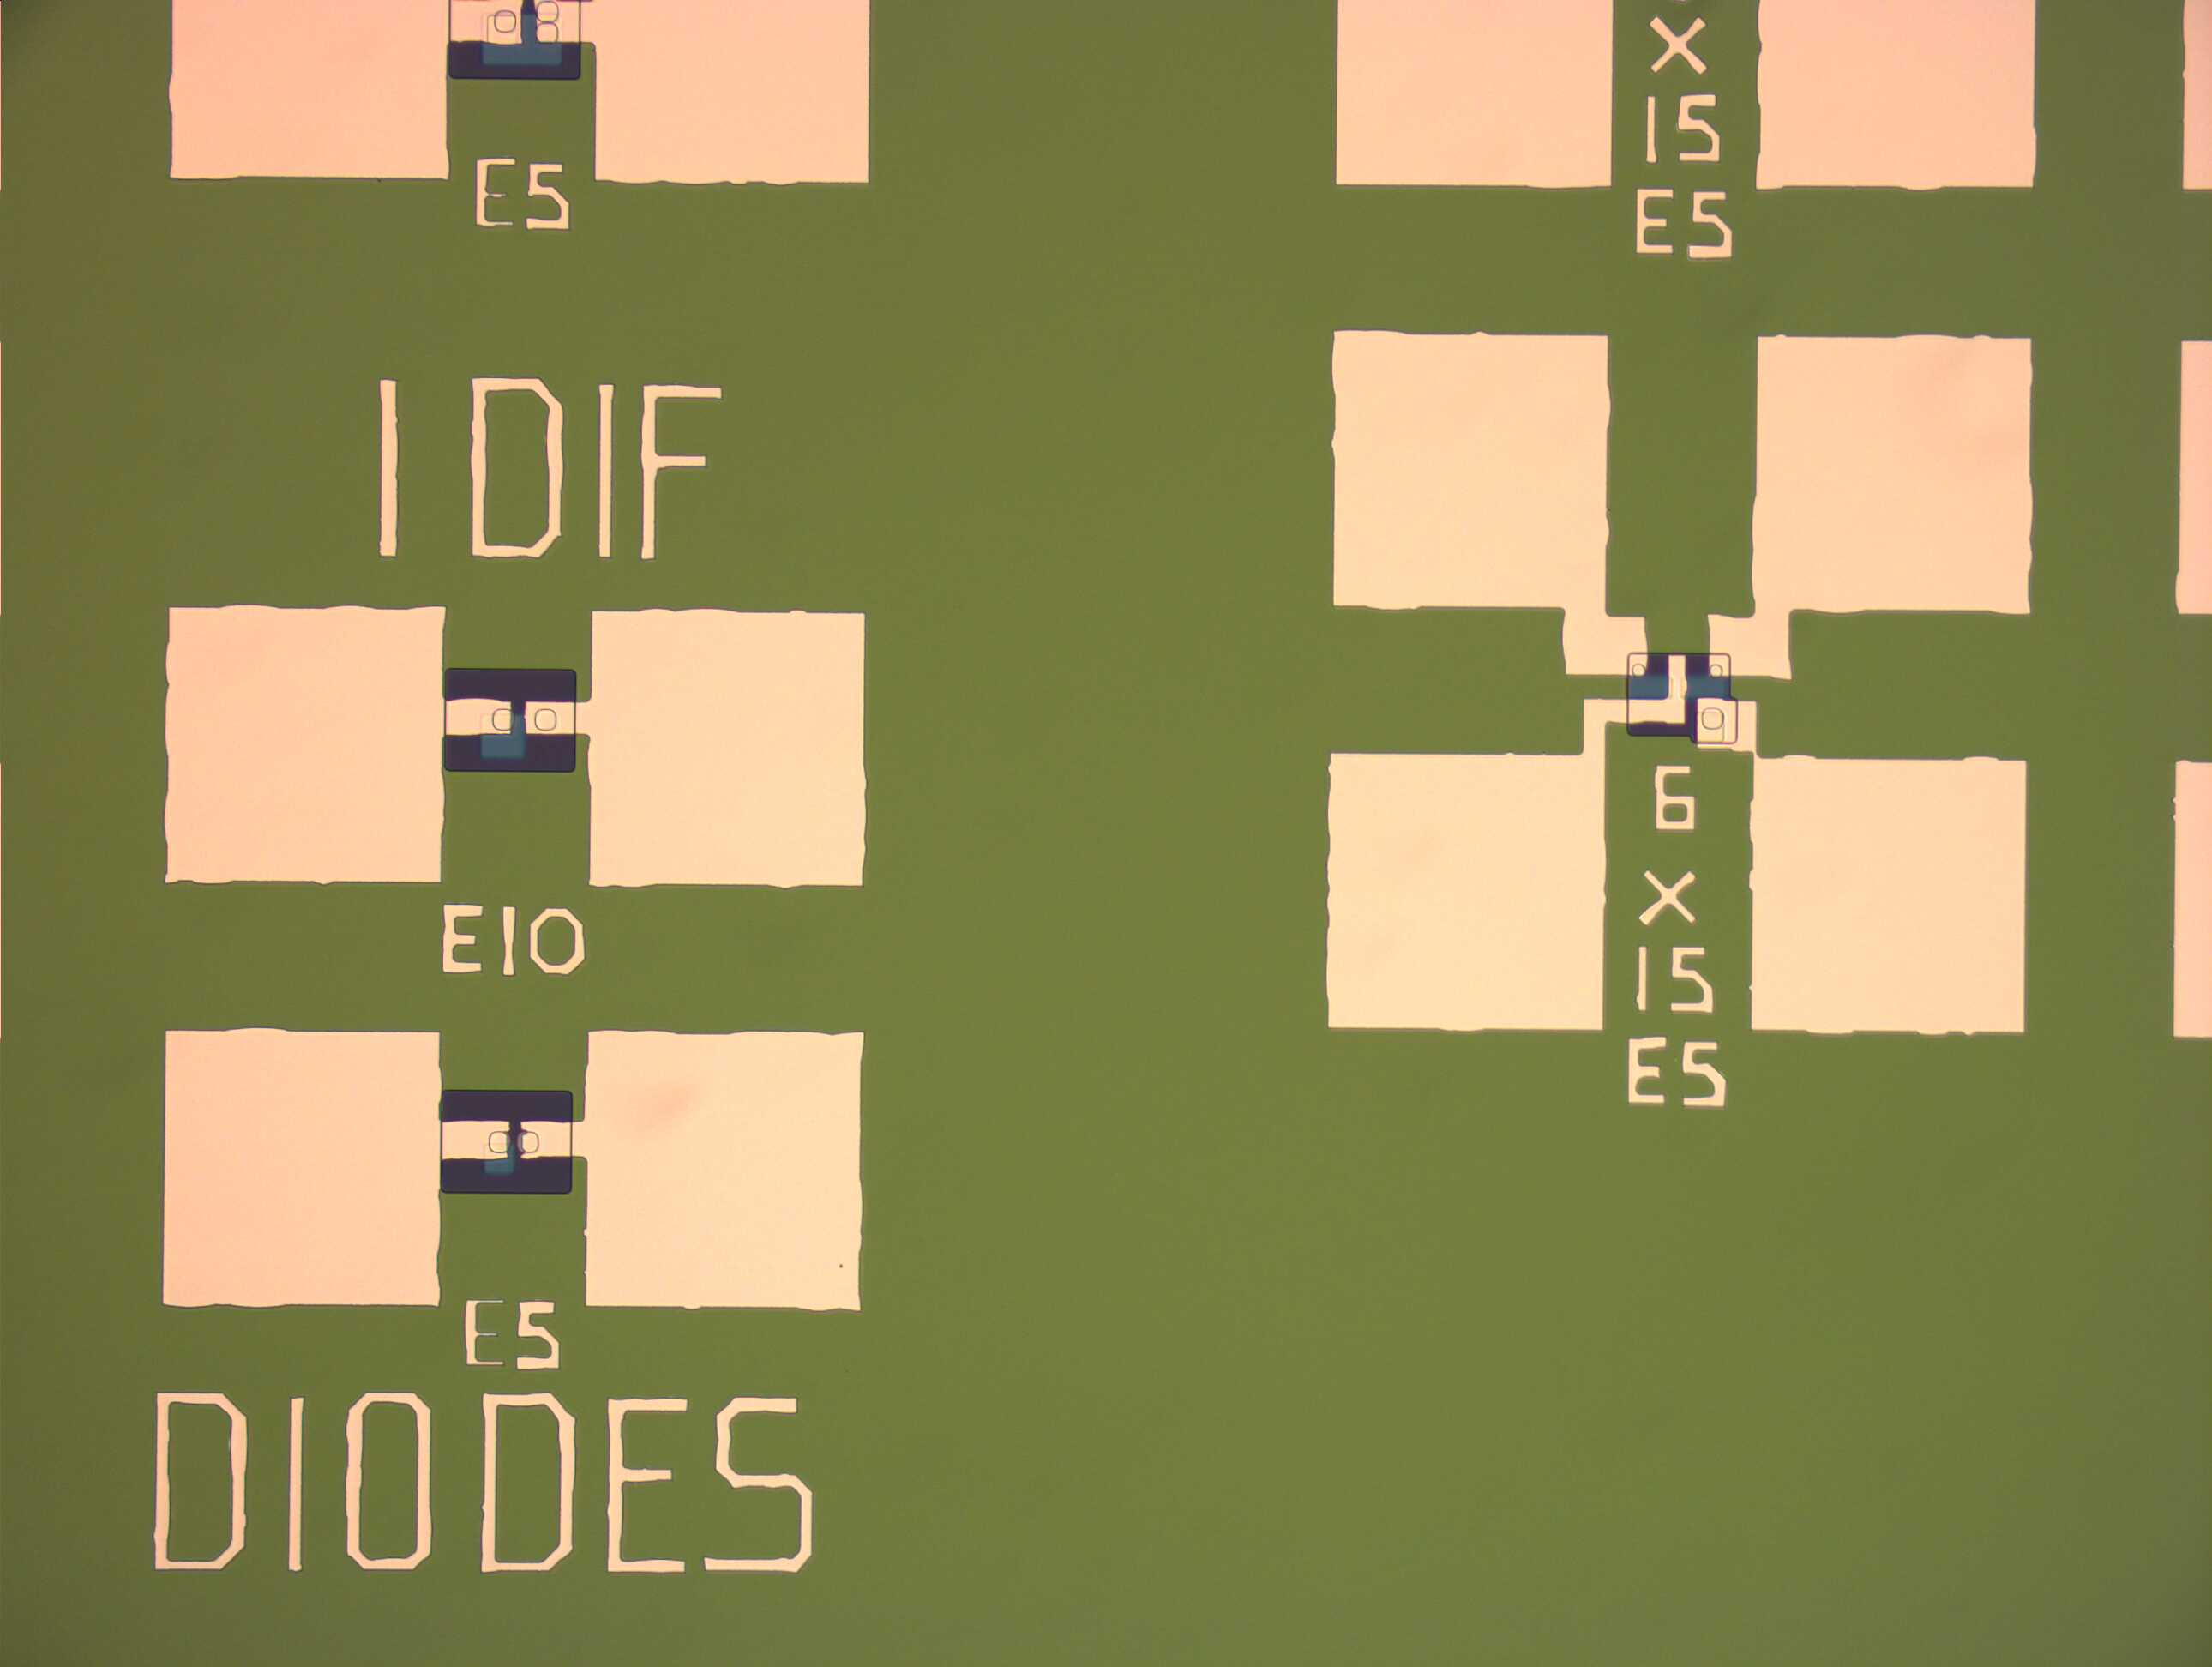
\includegraphics[width=.45\textwidth]{./Images/19_Nov_Diodes.jpg}
			\caption{Captured Image of Diodes}
			\label{fig:D_Image}
		\end{figure}
	
		\subsubsection{1 Diffusion}
			\FloatBarrier
			The 1 diffusion diodes in both the N$^-$ and P$^+$ regions are very similar.  The P$^+$ diode is the closer of the two to an ideal diode, as it has the steeper growth, but the N$^-$ diode still closely matches what we expect of a diode.
			
			\begin{figure}[h!]
				\centering
				\begin{subfigure}[b]{.45\textwidth}
					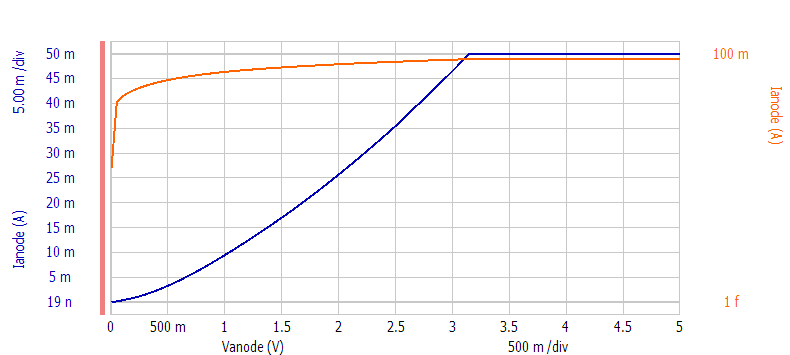
\includegraphics[width=\textwidth]{./Images/Probe_Test/D_Nwell_1diff.png}
					\caption{N$^-$ 1 Diffusion Diode}
				\end{subfigure}
				~
				\begin{subfigure}[b]{.45\textwidth}
					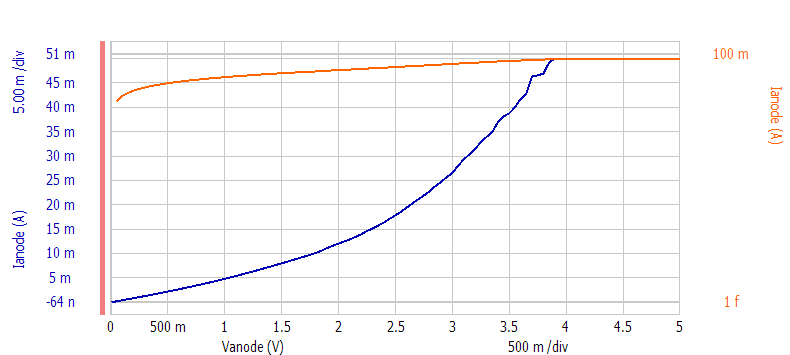
\includegraphics[width=\textwidth]{./Images/Probe_Test/D_Pwell_1diff.png}
					\caption{P$^+$ 1 Diffusion Diode}
				\end{subfigure}
				\caption{1 Diffusion Diodes}
				\label{fig:D_1diff}
			\end{figure}
		
		\subsubsection{2 Diffusion}
			\FloatBarrier
			For the 2 diffusion diodes, the N$^-$ diode closely resembles the 1 diffusion diode.  The P$^+$ diode however has a much steeper curve and a much earlier threshold voltage, closely matching what we expect of a real diode. This steeper curve is due to a comparatively lower resistance in the diode structure.
			\begin{figure}[]
				\centering
				\begin{subfigure}[b]{.45\textwidth}
					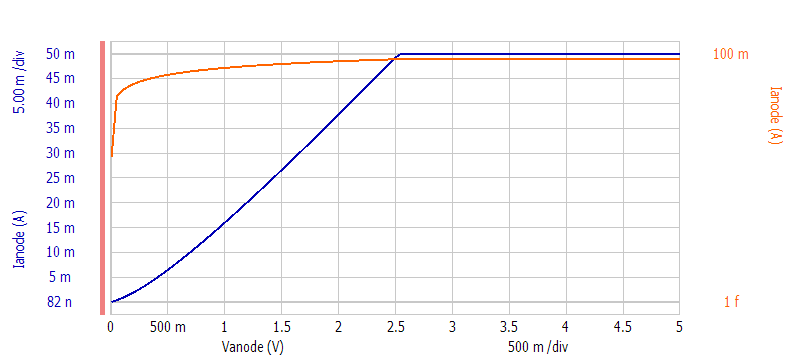
\includegraphics[width=\textwidth]{./Images/Probe_Test/D_Nwell_2diff.png}
					\caption{N$^-$ 2 Diffusion Diode}
				\end{subfigure}
				~
				\begin{subfigure}[b]{.45\textwidth}
					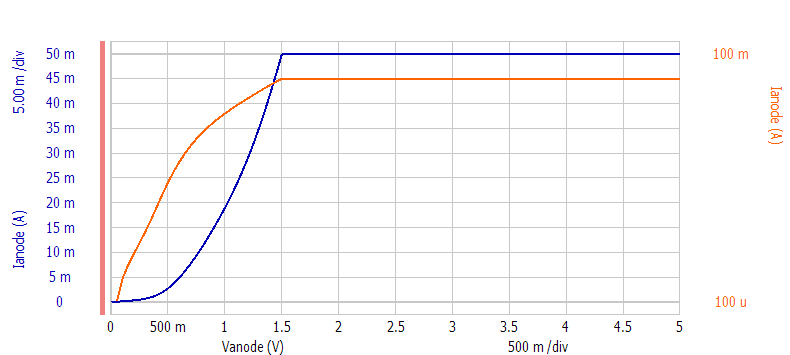
\includegraphics[width=\textwidth]{./Images/Probe_Test/D_Pwell_2diff.png}
					\caption{P$^+$ 2 Diffusion Diode}
				\end{subfigure}
				\caption{2 Diffusion Diodes}
				\label{fig:D_2diff}
			\end{figure}
	
	\FloatBarrier		
	\subsection{Transistors}\label{sec:Transistors}
		Figure~\ref{fig:T_Image} shows our transistors before and after the Al deposition step.
		
		\begin{figure}[h!]
			\centering
			\begin{subfigure}[b]{.45\textwidth}
				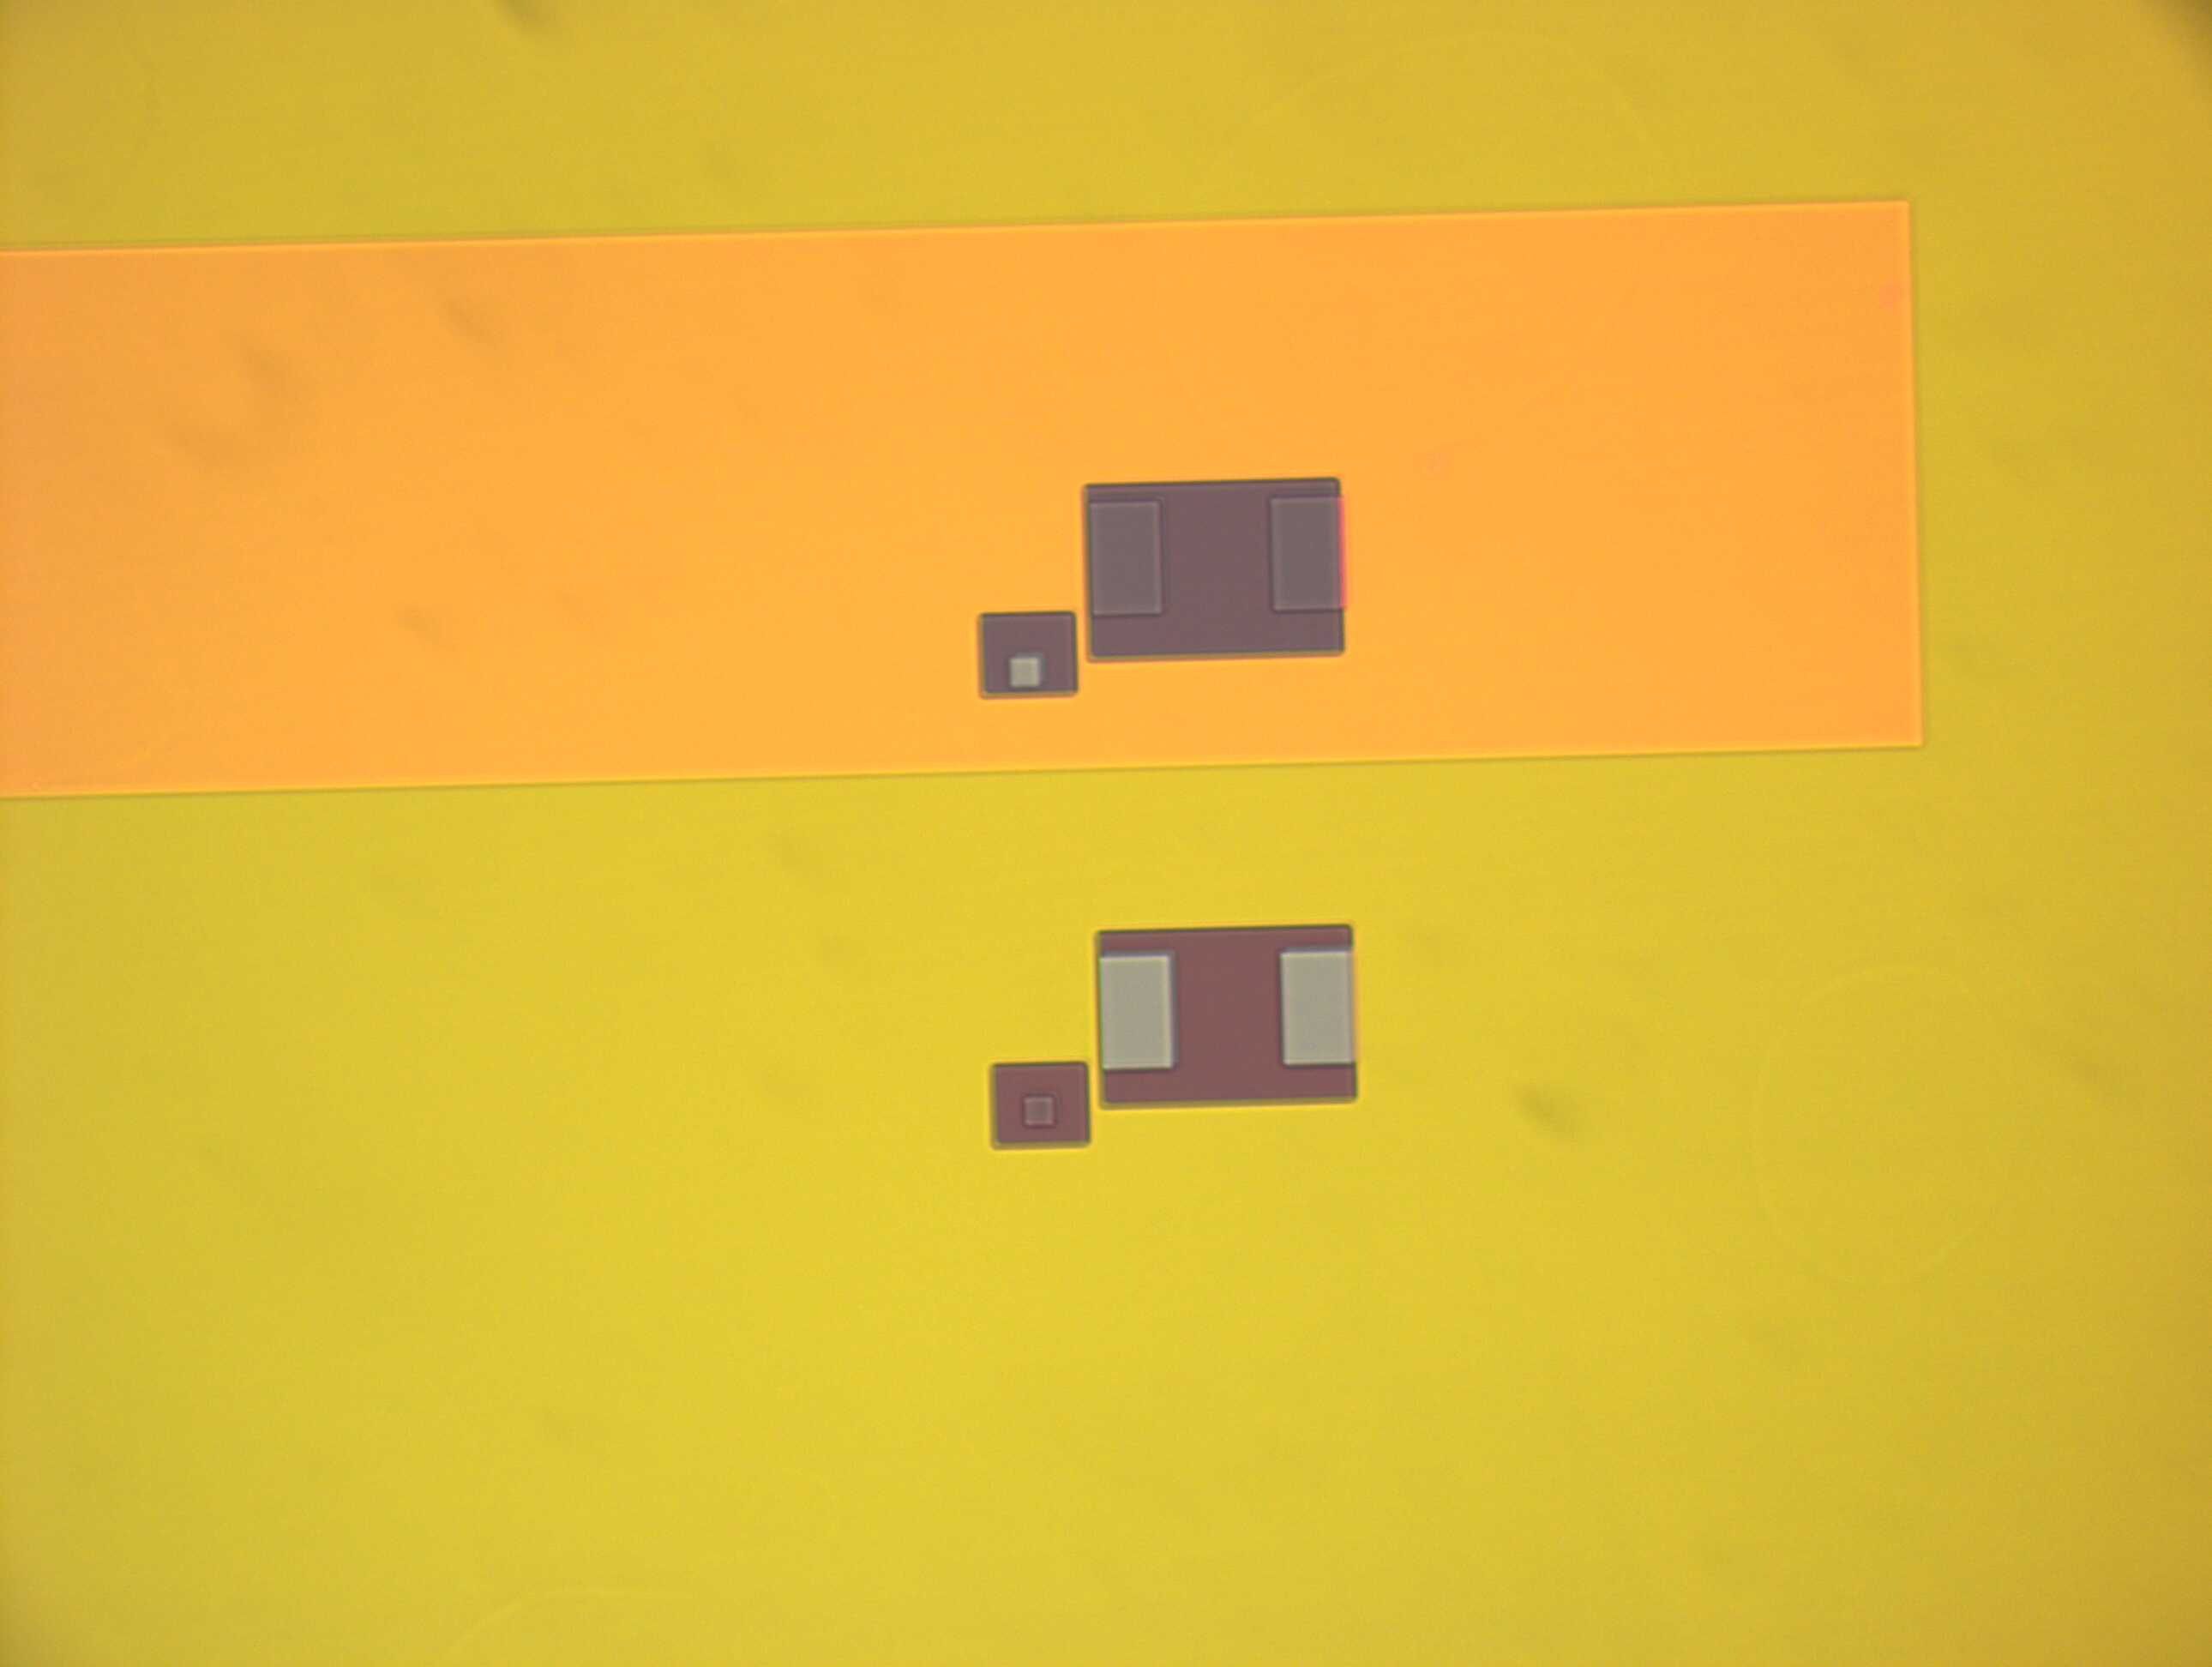
\includegraphics[width=\textwidth]{./Images/5_Nov_Transistors.jpg}
				\caption{Transistors before Al Deposition}
			\end{subfigure}
			~
			\begin{subfigure}[b]{.45\textwidth}
				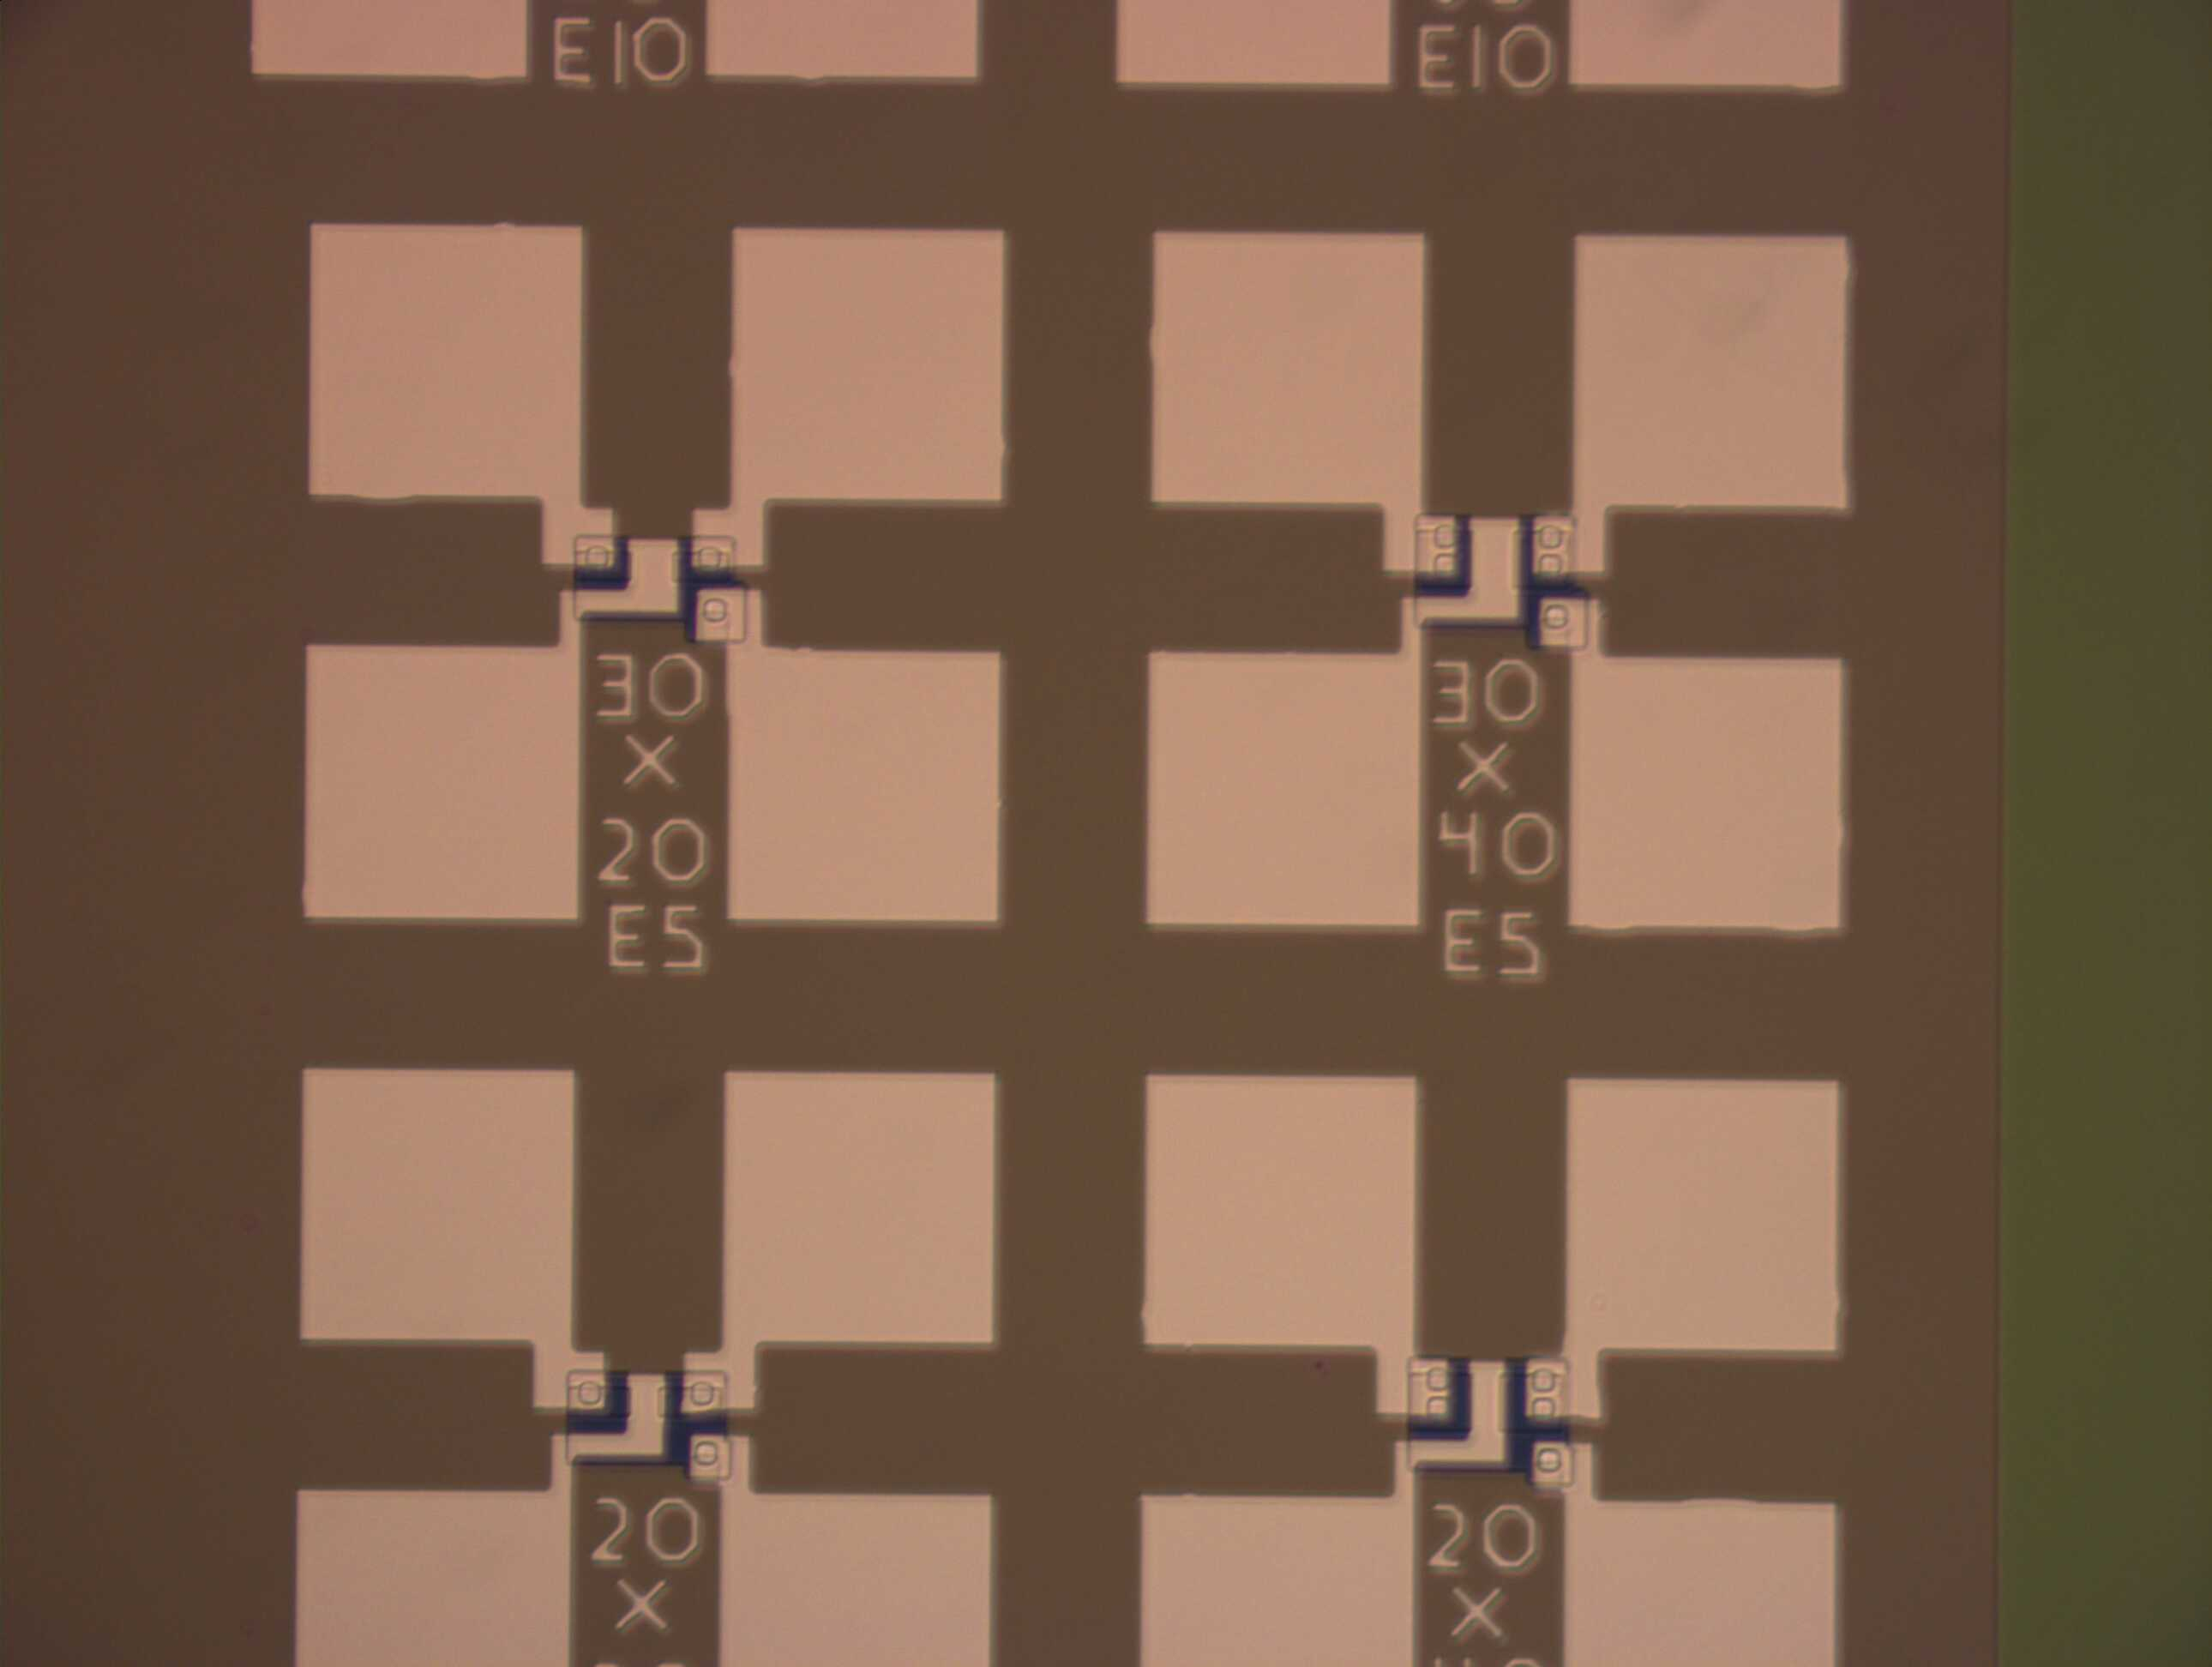
\includegraphics[width=\textwidth]{./Images/19_Nov_Transistors.jpg}
				\caption{Transistors after Al Deposition}
			\end{subfigure}
			\caption{Capture Images of Transistors}
			\label{fig:T_Image}
		\end{figure}
	
		\FloatBarrier
		\subsubsection{NMOS}
			Unfortunately, I was unable to find any working NMOS transistors on the entire wafer.  The transistor operates the same regardless of the gate bias voltage.  As can be seen in Figure~\ref{fig:T_NMOS}, the transistor response most closely resembles a diode with an extremely high threshold voltage, at which point the current quickly reaches the tester's current limit. As we can clearly see the presence of Al over the gate region of the transistor, the gate oxide must be much thicker than expected.
			
			\begin{figure}[h!]
				\centering
				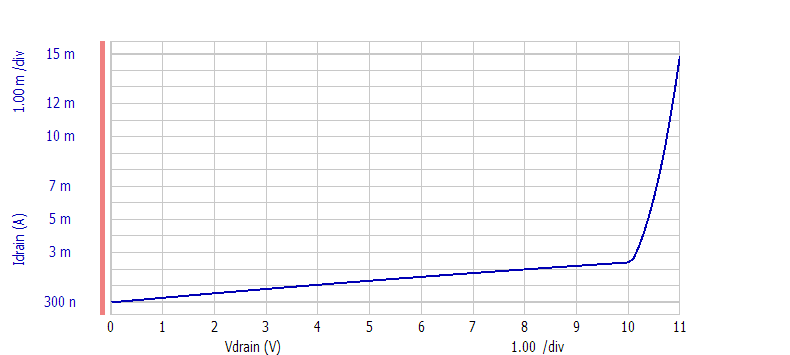
\includegraphics[width=\textwidth]{./Images/Probe_Test/T_NMOS_190x160E10.png}
				\caption{A NMOS transistor 190x160}
				\label{fig:T_NMOS}
			\end{figure}
		
		\FloatBarrier
		\subsubsection{PMOS}
			Similar to the NMOS transistors, I was unable to find any working PMOS transistors, and the gate bias voltage has no effect on their operation.  As can be seen in Figure~\ref{fig:T_PMOS}, the transistor response most closely resembles a resistor of approximately 62.5 $\Omega$. The resistor behavior could be explained by extreme lateral diffusion, connecting the source and drain diffusions together.  This would also theoretically negate the any gate bias, though it is like that the gate oxide is the same thickness as on the NMOS transistors.
			
			\begin{figure}[h!]
				\centering
				\includegraphics[width=\textwidth]{./Images/Probe_Test/T_PMOS_190x160E10.png}
				\caption{A PMOS transistor 190x160}
				\label{fig:T_PMOS}
			\end{figure}
			
\FloatBarrier
\section{Results}
	As previously stated in Section~\ref{sec:Transistors}, there were no working transistors on the wafer.  This is likely due to a thicker than expected gate oxide.  Whether the oxide is too thick because we did not manage to strip away the field oxide before growing the gate oxide or the gate oxidation was insufficient is unknown.  The PMOS transistors also behaved as resistors, suggesting that the P$^+$ Source and Drain were connected. This effect may be due to excess lateral diffusion of the P$^+$ dopant.
	
	\subsection{Recommendations}
		The PMOS errors could have been due to the 'experiment' of this year's class.  Our lab section used 10 min of Nitrogen followed by 10 min of Oxygen during the deposition of the N$^-$ well. Traditionally, the PMOS transistors have been difficult to make work, so further experimentation is the recommended course of action.
		
		Personally, I wasn't sure what I was looking for whenever we looked at the wafer until the aluminum was deposited.  Similar to how the entire process (N$^-$ well, N$^+$ Source \& Drain, P$^+$ Source \& Drain, Gate, Contacts) is often repeated in class, it might be helpful to throw up a picture of the wafer/die before lab sections so students might understand what they are looking at under a microscope.

\pagebreak
\printbibliography

\end{document}